\addcontentsline{toc}{chapter}{\textbf{Anexo 1}} 
\lhead{Anexo 1}
\rhead{\newtitle}
\cfoot{\thepage}
\renewcommand{\headrulewidth}{1pt}
\renewcommand{\footrulewidth}{1pt}

\chapter*{Anexo 2}


\noindent \textbf{Mapas de GHI derivados del proceso de adaptación al sitio}.

Una de las herramientas ampliamente en la caracterización del recurso solar son sin dudas los mapas que explican de manera rápida e intuitiva de cómo distribuye el recurso en una región. La construcción de estos ha sido ampliamente estudiada en diversas partes del mundo debido a su utilidad en distintas áreas de aplicaciones. Particularmente en Argentina dentro de la Guía del Recurso Solar publicada por la Secretaría de Energía se distribuye el ATLAS DE ENERGÍA SOLAR DE LA REPÚBLICA ARGENTINA que indica la distribución espacial del promedio de la irradianción solar global diaria sobre un plano horizontal discriminada por mes trazándose las isolíneas correspondientes a cada mes y al año
espaciadas 0.5 kWh/m2. Una aproximación de esto implementada para el Noroeste Argentino es el TRAZADO DE MAPAS MEDIOS ANUALES DE ENERGÍA SOLAR GLOBAL, DIRECTA, DIFUSA Y TILT, USANDO LA BASE DE DATOS DE SWERA. CASO DE ESTUDIO: PROVINCIAS DE SALTA Y JUJUY. Donde se presentan mapas de líneas de iso-irradiación solar global media anual para las provincias de Salta y Jujuy utilizando los datos dela base satelital SWERA, cuyas celdas son cuadrados de 40 km. de lado, a través del método geoestadístico del kriging y un variograma lineal. 


Además de la utilidad evidente de los mapas mensuales de irradiación, resulta imprescindible incorporar un Año Meteorológico Típico (TMY, por sus siglas en inglés) como insumo fundamental para la caracterización robusta del recurso solar. El TMY permite condensar en un solo año sintético las condiciones climáticas representativas de un período histórico más extenso, evitando que la evaluación dependa de anomalías o eventos extremos propios de años particulares. Esta aproximación garantiza que los análisis derivados —ya sean energéticos, estadísticos o de diseño— se apoyen en una base climatológica estable y científicamente defendible.

El empleo de un TMY contribuye, asimismo, a mejorar la comparabilidad de los resultados entre regiones y entre distintos estudios. Dado que constituye un estándar internacionalmente aceptado en la industria solar, su utilización asegura que la interpretación de los mapas y métricas derivadas no se vea afectada por variaciones interanuales propias de la dinámica atmosférica. En consecuencia, los mapas mensuales construidos a partir de un TMY adquieren una mayor validez para estudios de planificación y apoyo a políticas públicas.


La construcción del TMY fue realizado exclusivamente a partir de la GHI, como el obtenido mediante el método de Finkelstein–Schafer con procesamiento vectorizado, constituye un paso metodológico plenamente válido y científicamente justificado cuando el objetivo central es la caracterización espacial del recurso solar. La GHI sintetiza la mayor parte de la variabilidad radiativa relevante para estudios de disponibilidad energética, por lo que disponer de un TMY específico para esta variable permite estabilizar dicha variabilidad y evitar que los mapas mensuales se vean distorsionados por fluctuaciones episódicas asociadas a años inusualmente nublados o excepcionalmente despejados. Esto adquiere especial relevancia en regiones subtropicales o de topografía compleja, donde la variabilidad interanual puede ser significativa.

El uso del método Finkelstein–Schafer para la selección del TMY garantiza que el año sintético conserve, para cada mes, la forma estadística de la distribución horaria de GHI, reproduciendo fielmente las colas, percentiles y patrones de dispersión que caracterizan al clima local. Este enfoque es particularmente robusto cuando se trabaja con series extensas y heterogéneas, como las derivadas de bases satelitales corregidas, y es compatible con la construcción de productos espaciales como mapas mensuales, dado que preserva la coherencia entre celdas y evita la introducción de discontinuidades artificiales. Por ello, aun con una única variable radiativa, el TMY aporta una base homogénea sobre la cual montar comparaciones y análisis espaciales.

Además, la necesidad de un TMY se intensifica al trabajar con interpolaciones espaciales o con métodos geoestadísticos —como kriging sobre mallas satelitales—, ya que estos algoritmos dependen críticamente de la estabilidad estadística de los datos de entrada. En ausencia de un TMY, un año particular podría inducir gradientes irreales o sesgos en las isolíneas mensuales, comprometiendo la interpretación de los patrones de irradiación. En contraste, un TMY asegura que los mapas reflejen la climatología promedio y no el comportamiento anómalo de un subconjunto temporal limitado. De este modo, se mejora la calidad cartográfica y se preserva la relevancia física de las estructuras espaciales observadas.

Asimismo, la integración del TMY con la metodología de site adaptation —previamente discutida— permite extender de forma consistente los resultados hacia regiones con escasa instrumentación o alta dependencia de datos satelitales corregidos. El TMY actúa como un marco de referencia climatológico uniforme que facilita compatibilizar las adaptaciones por sitio con la estructura estadística regional, evitando que cada mapa mensual responda a patrones temporales idiosincráticos que dificulten su comparación transversal. Esto se traduce en una herramienta más robusta para estudios de sensibilidad, validación regional y análisis de desempeño energético.

Finalmente, la generación de los doce mapas mensuales de GHI media basados en el TMY obtenido no solo preserva la representatividad climatológica del recurso, sino que también proporciona una base metodológica sólida para estudios comparativos, planificación energética y análisis de potencial solar. De este modo, los mapas presentados se apoyan en una estructura temporal sintetizada que retiene las características más recurrentes y fundamentales del clima radiativo regional, cumpliendo con los estándares habituales de la literatura internacional en recursos solares y reforzando la credibilidad científica de los productos cartográficos derivados.



A continuación se presentan los doce mapas mensuales de la Irradiación Global Horizontal (GHI) obtenidos a partir del Año Meteorológico Típico (TMY), resultantes del proceso de adaptación al sitio.

\begin{figure}[H]
\centering
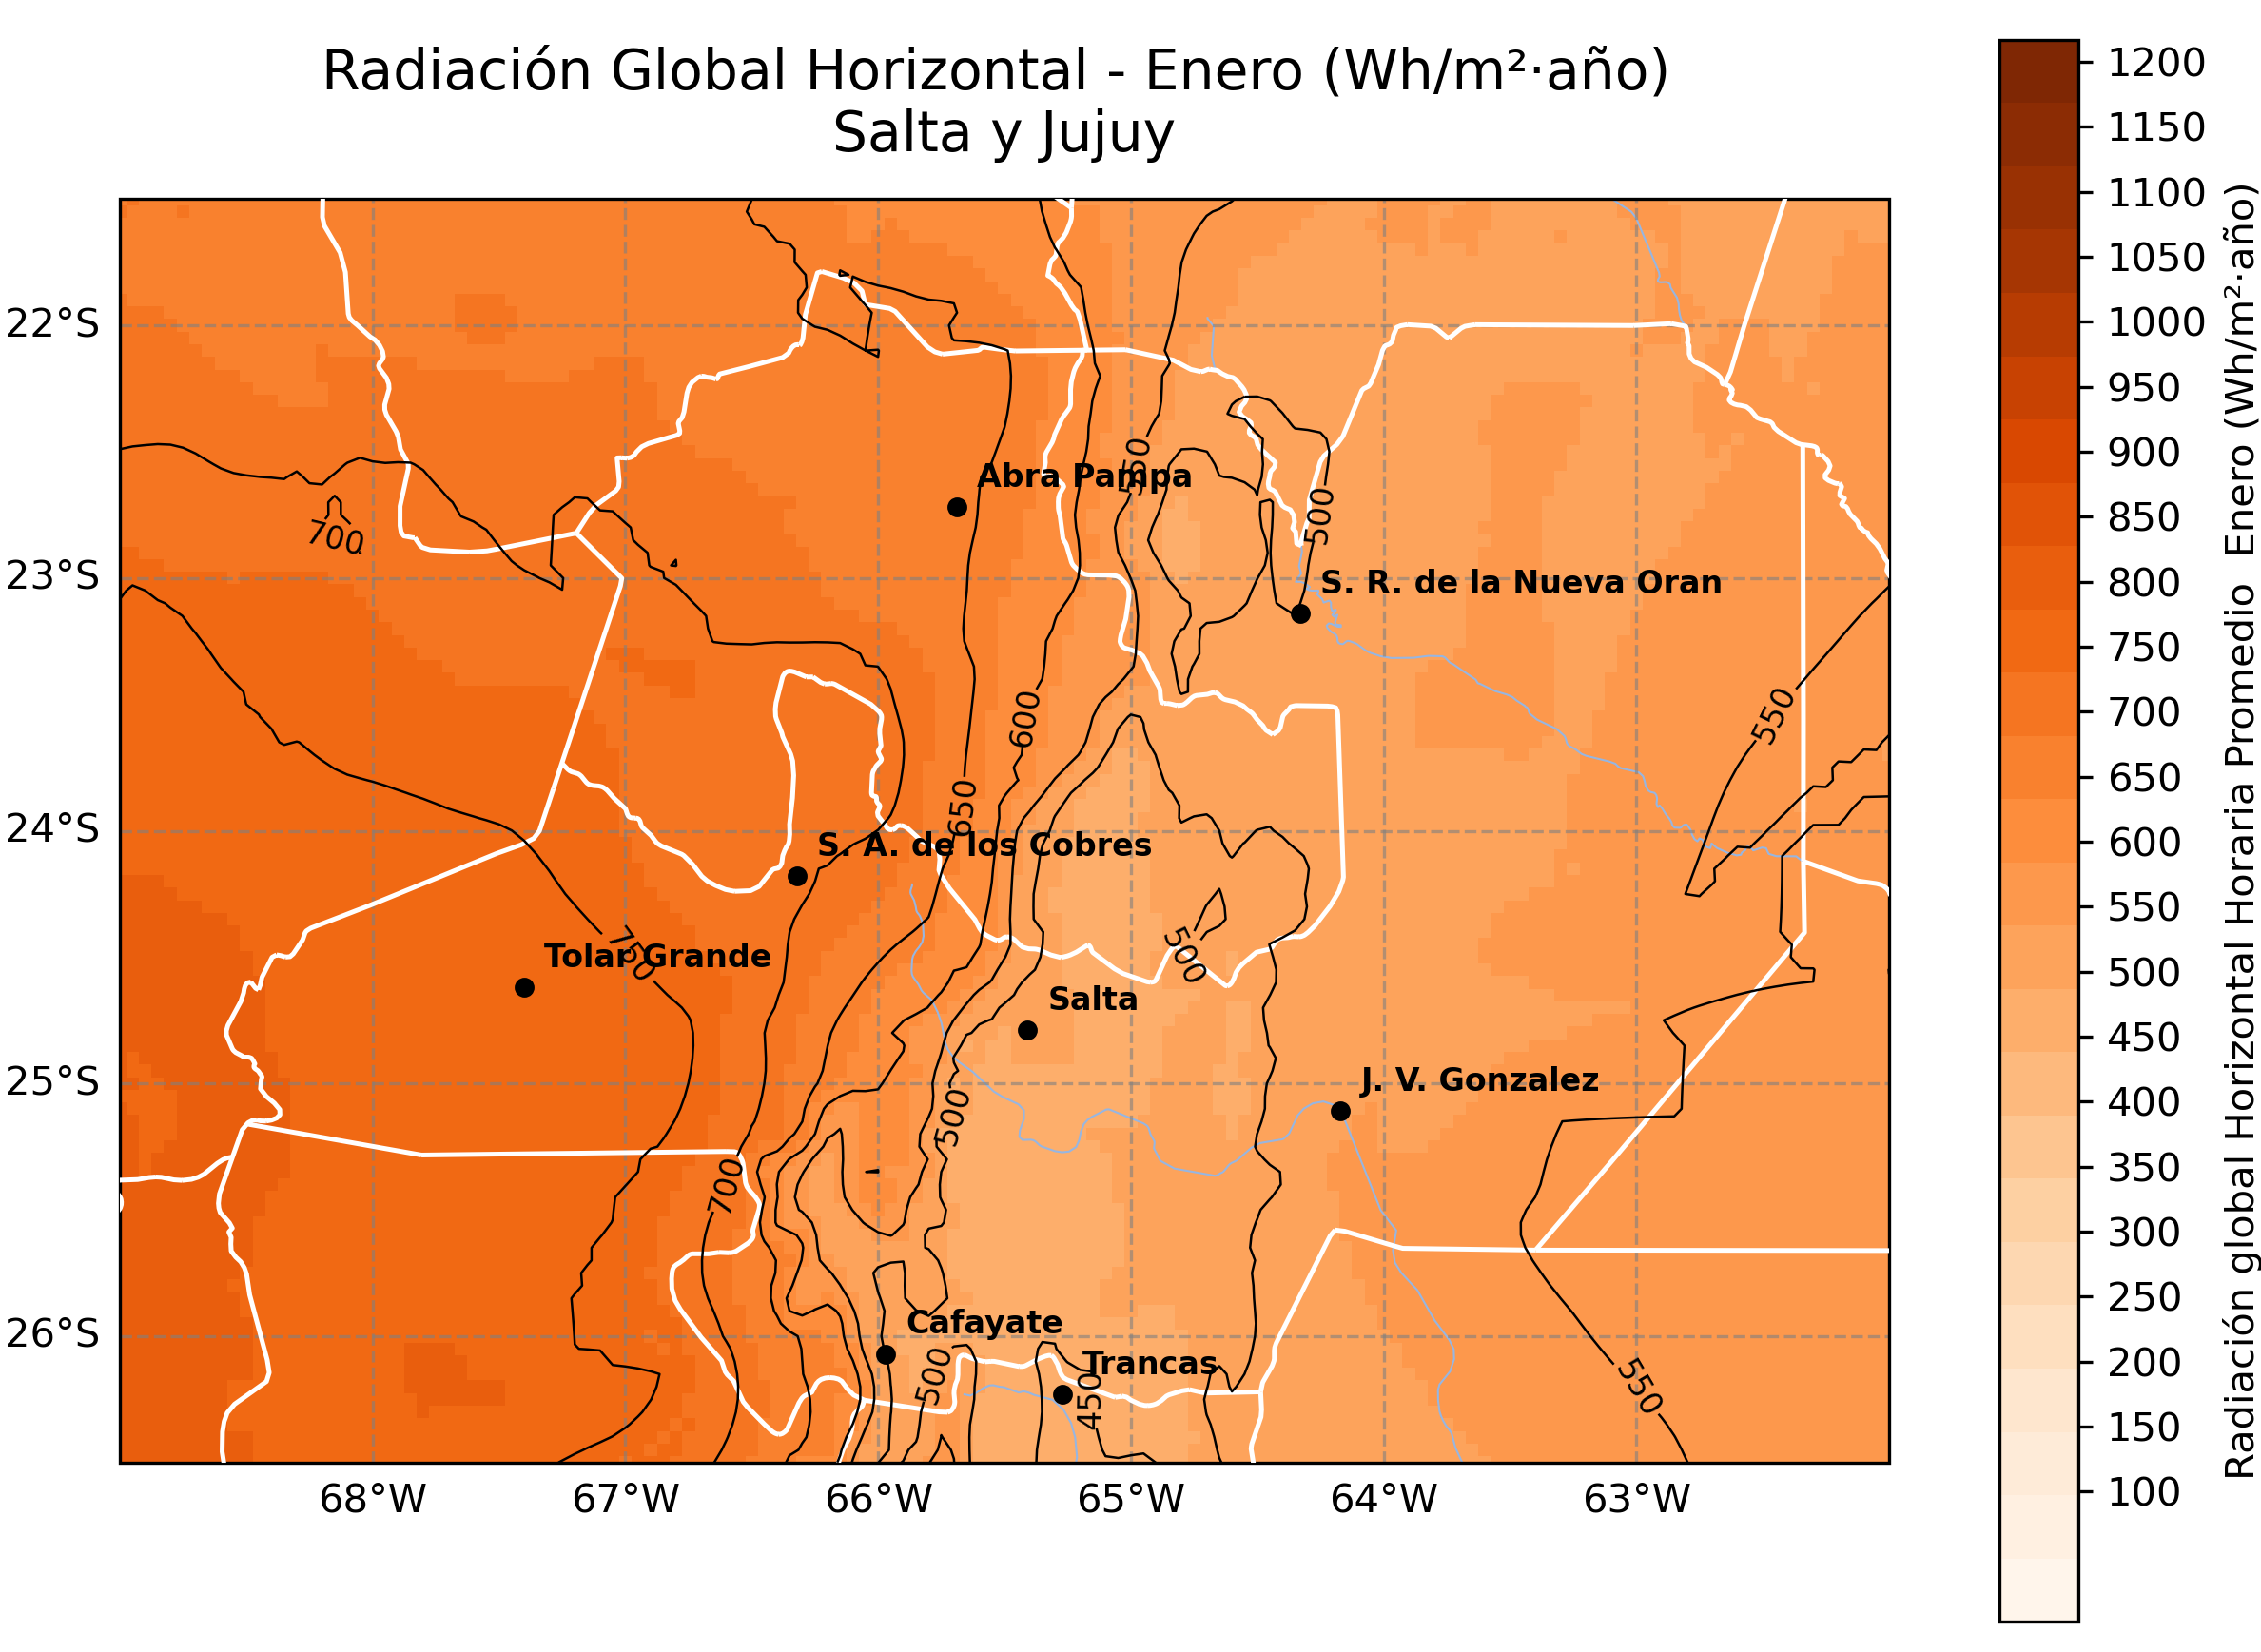
\includegraphics[width=0.95\textwidth]{figuras/Mapas/1_Enero.png}
\caption{Mapa de GHI medio mensual – Enero (TMY).}
\end{figure}

\begin{figure}[H]
\centering
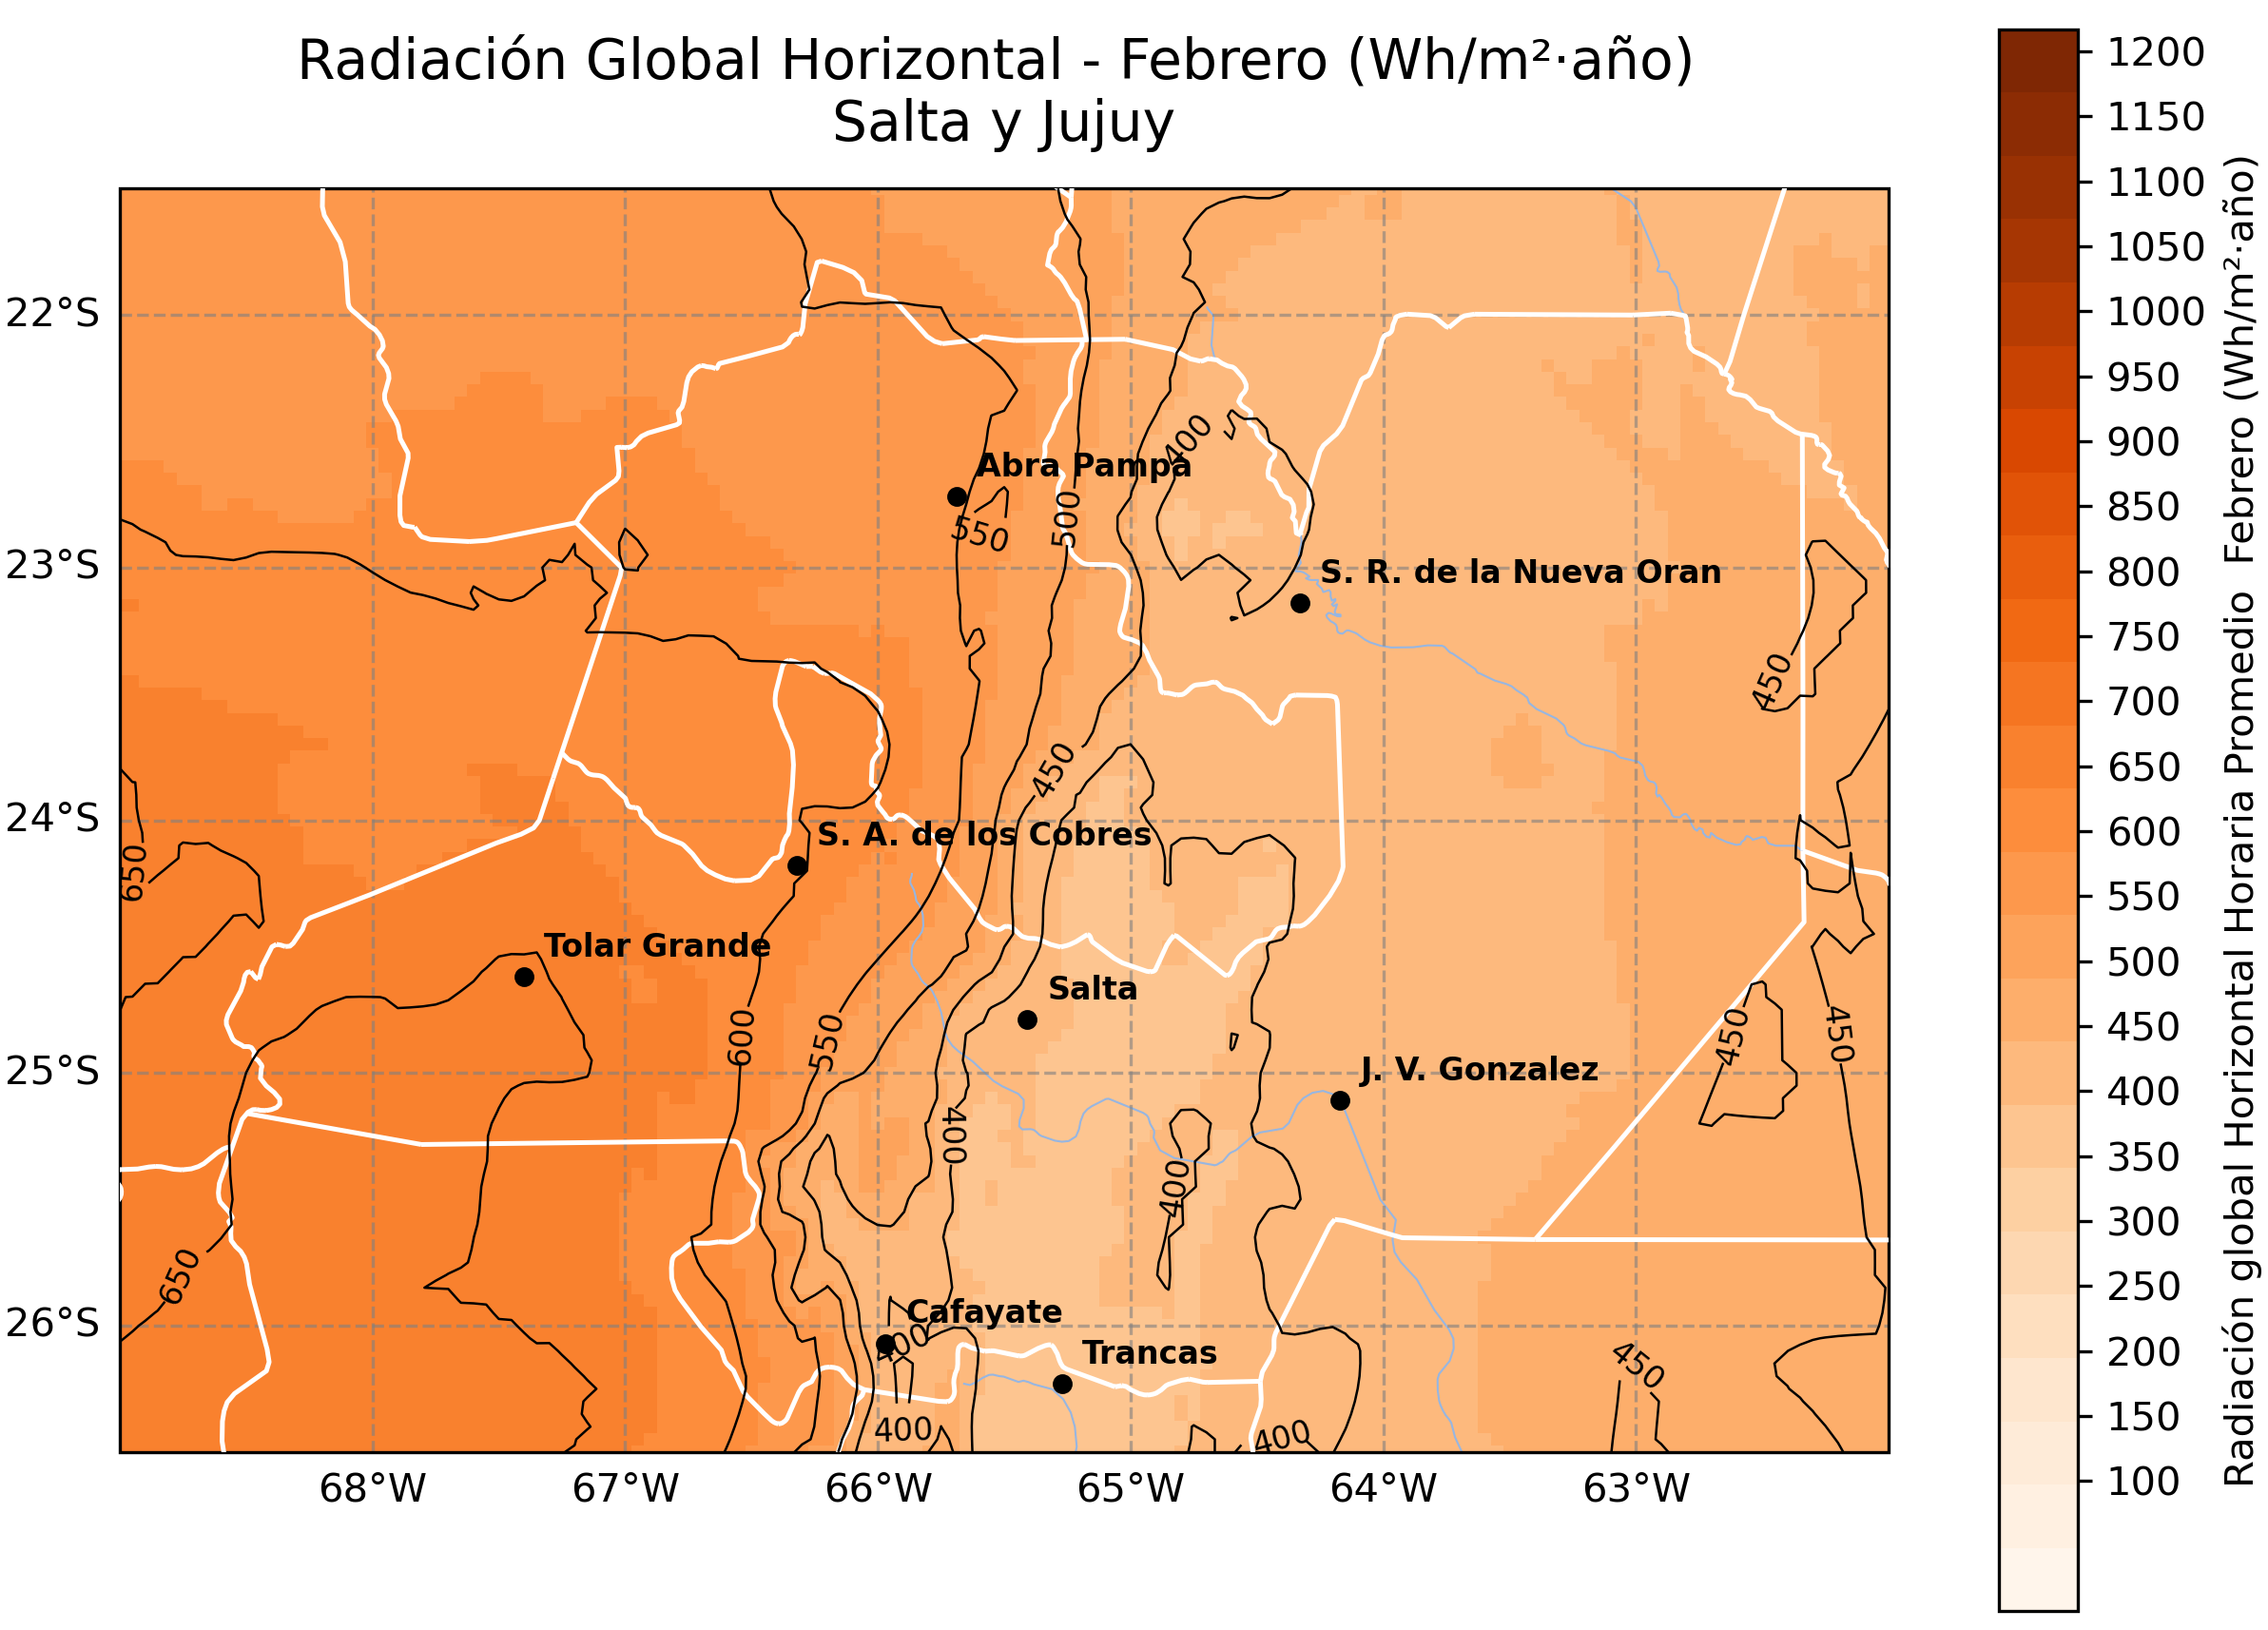
\includegraphics[width=0.95\textwidth]{figuras/Mapas/2_Febrero.png}
\caption{Mapa de GHI medio mensual – Febrero (TMY).}
\end{figure}

\begin{figure}[H]
\centering
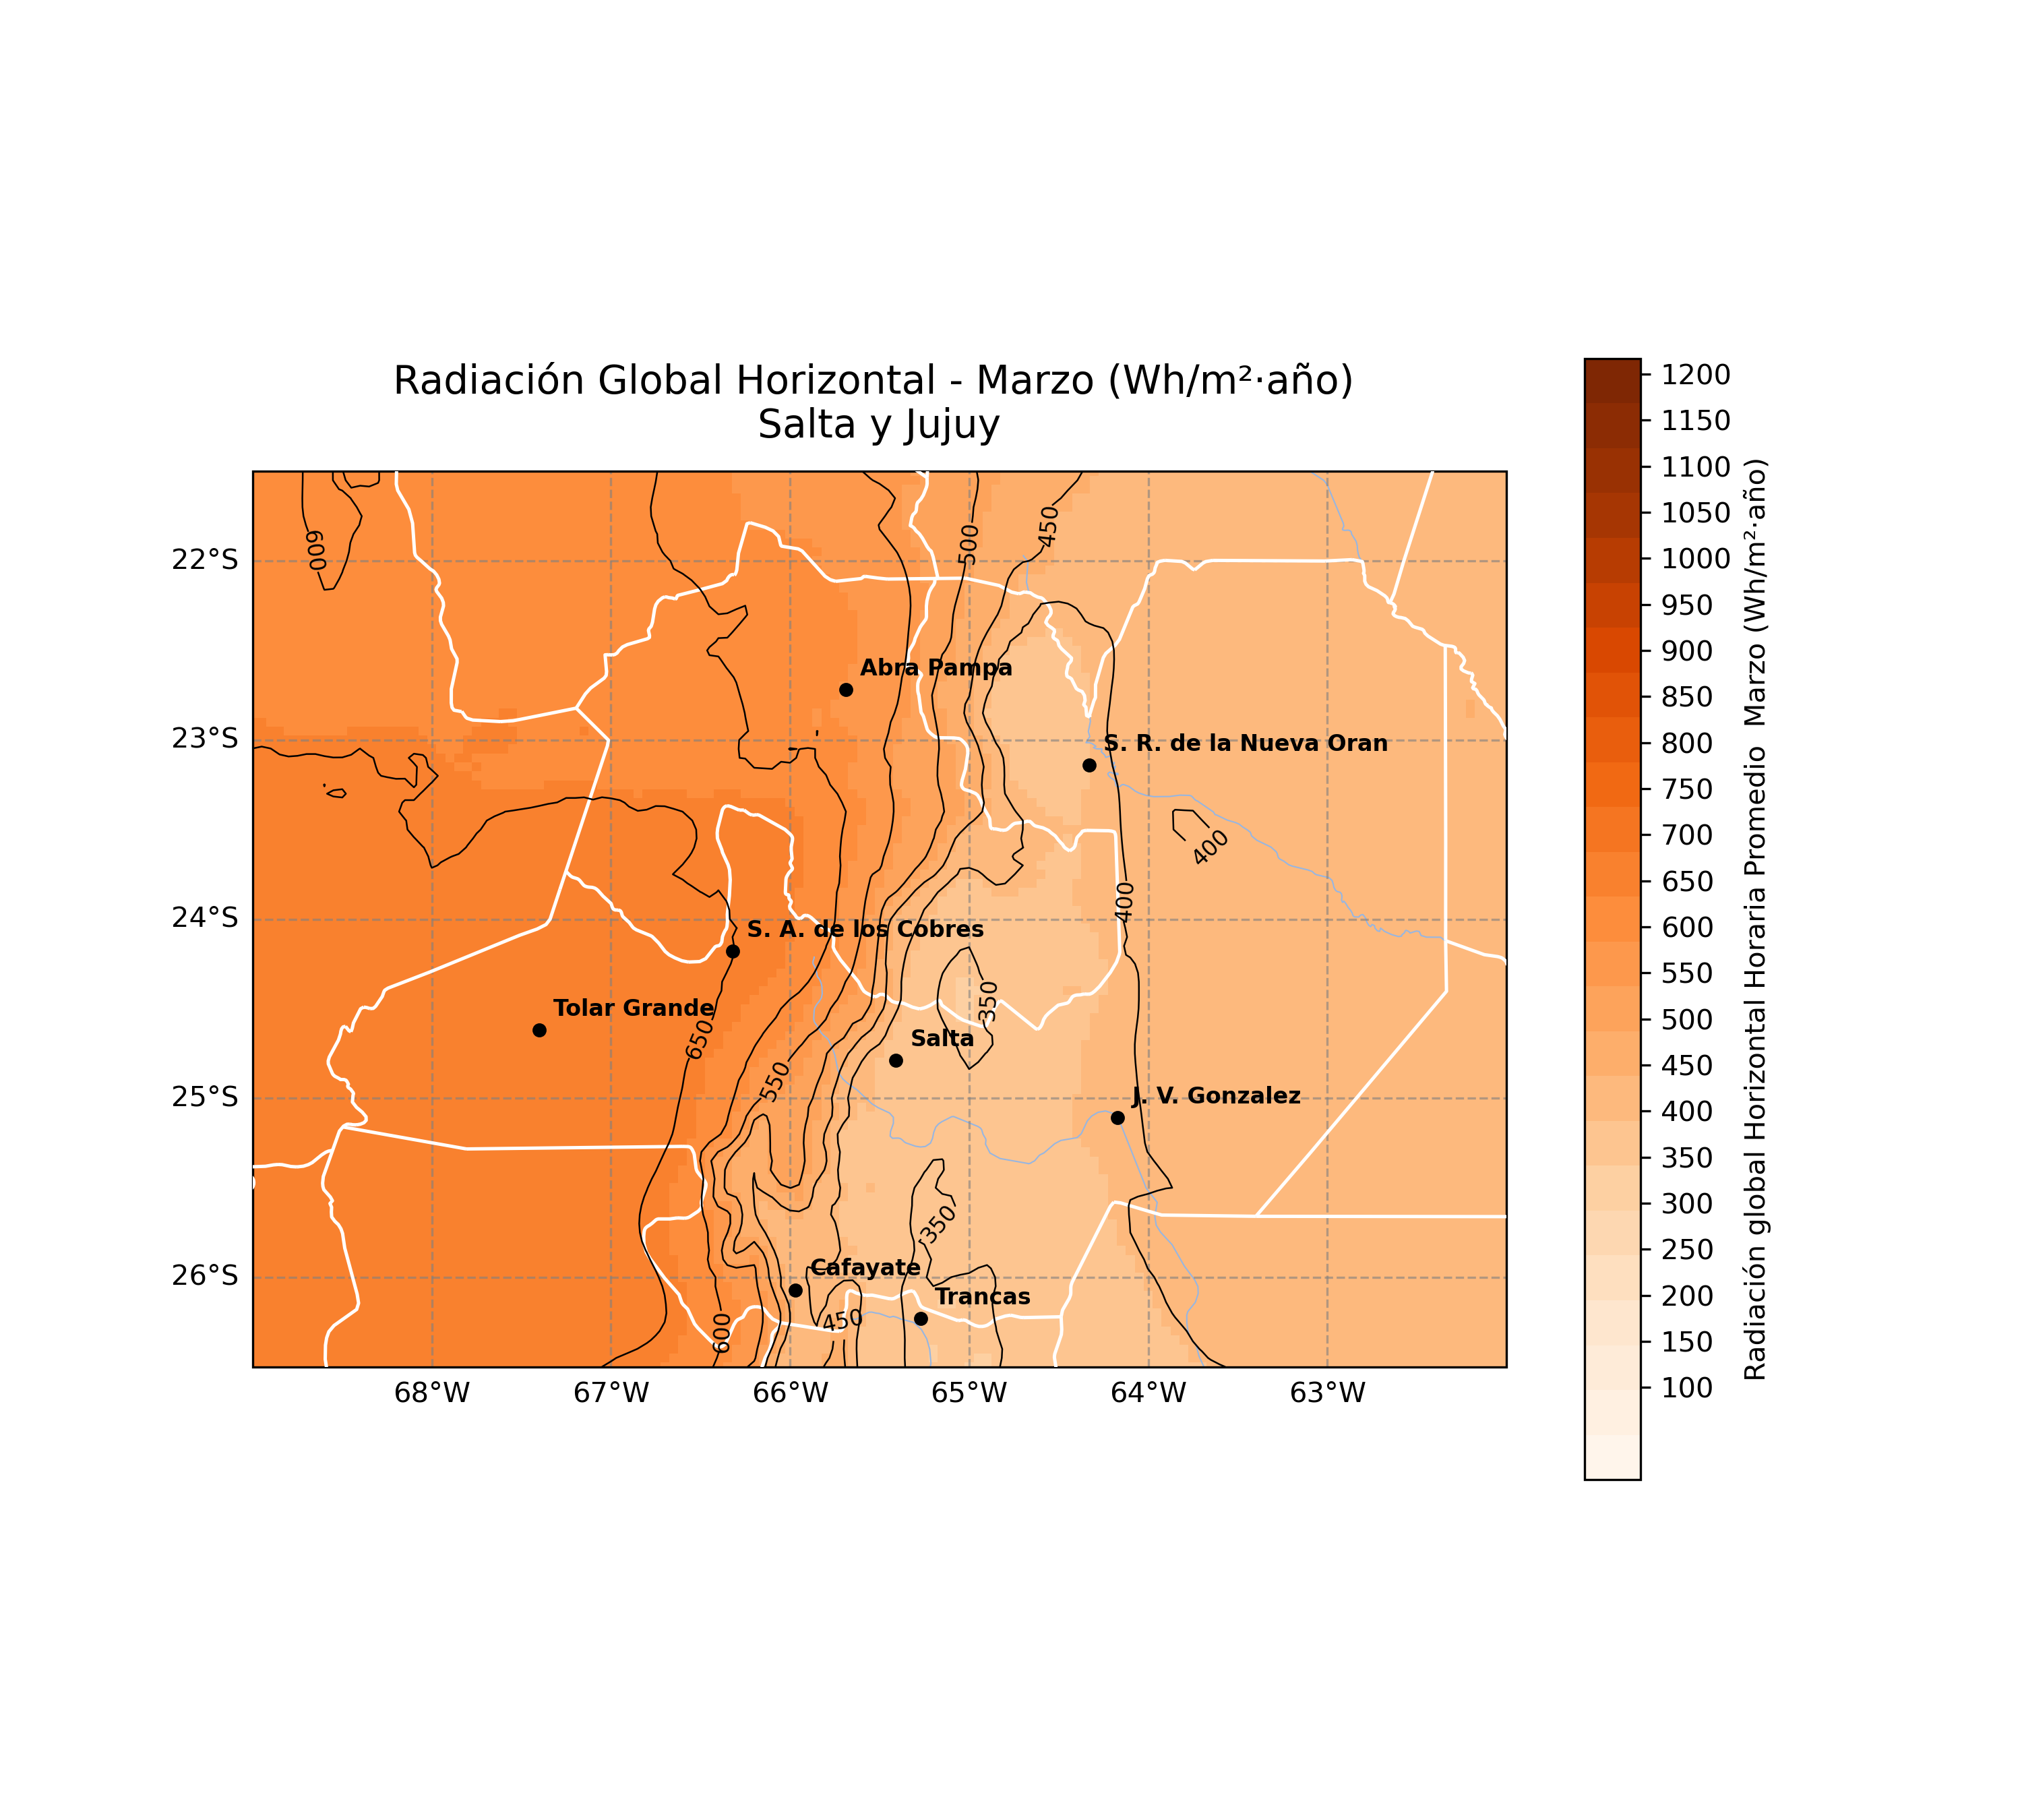
\includegraphics[width=0.95\textwidth]{figuras/Mapas/3_Marzo.png}
\caption{Mapa de GHI medio mensual – Marzo (TMY).}
\end{figure}

\begin{figure}[H]
\centering
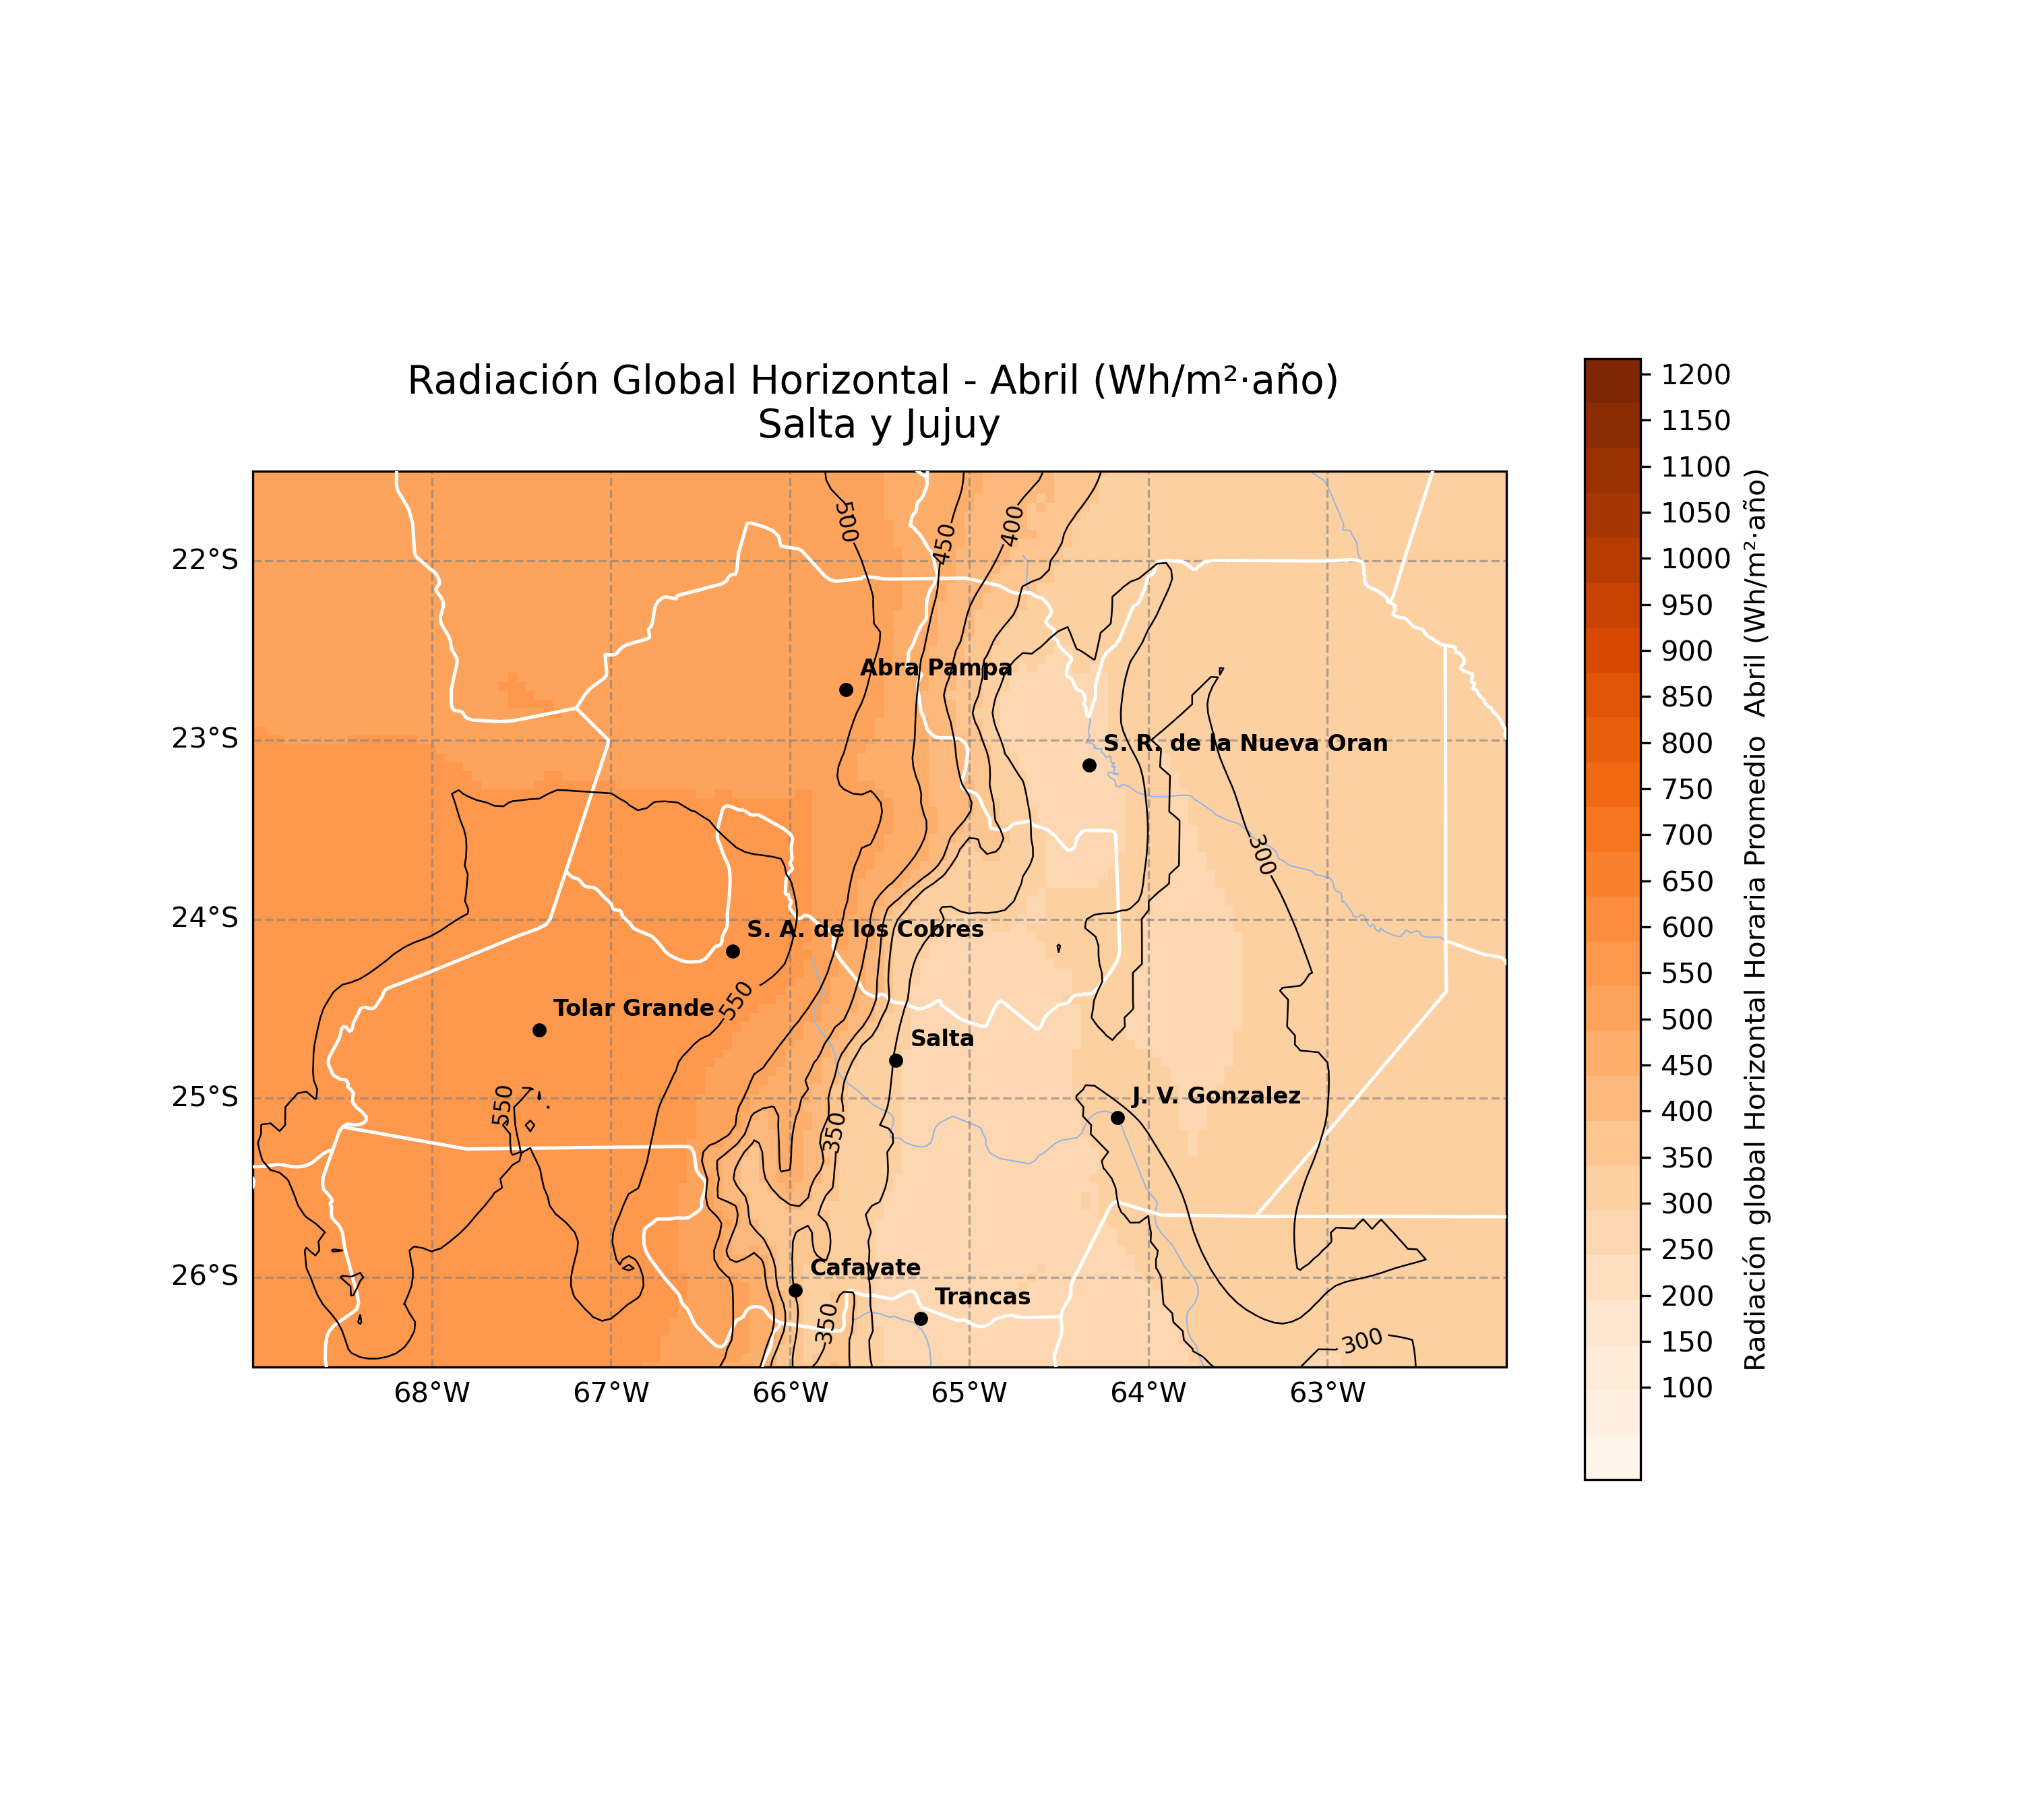
\includegraphics[width=0.95\textwidth]{figuras/Mapas/4_Abril.png}
\caption{Mapa de GHI medio mensual – Abril (TMY).}
\end{figure}

\begin{figure}[H]
\centering
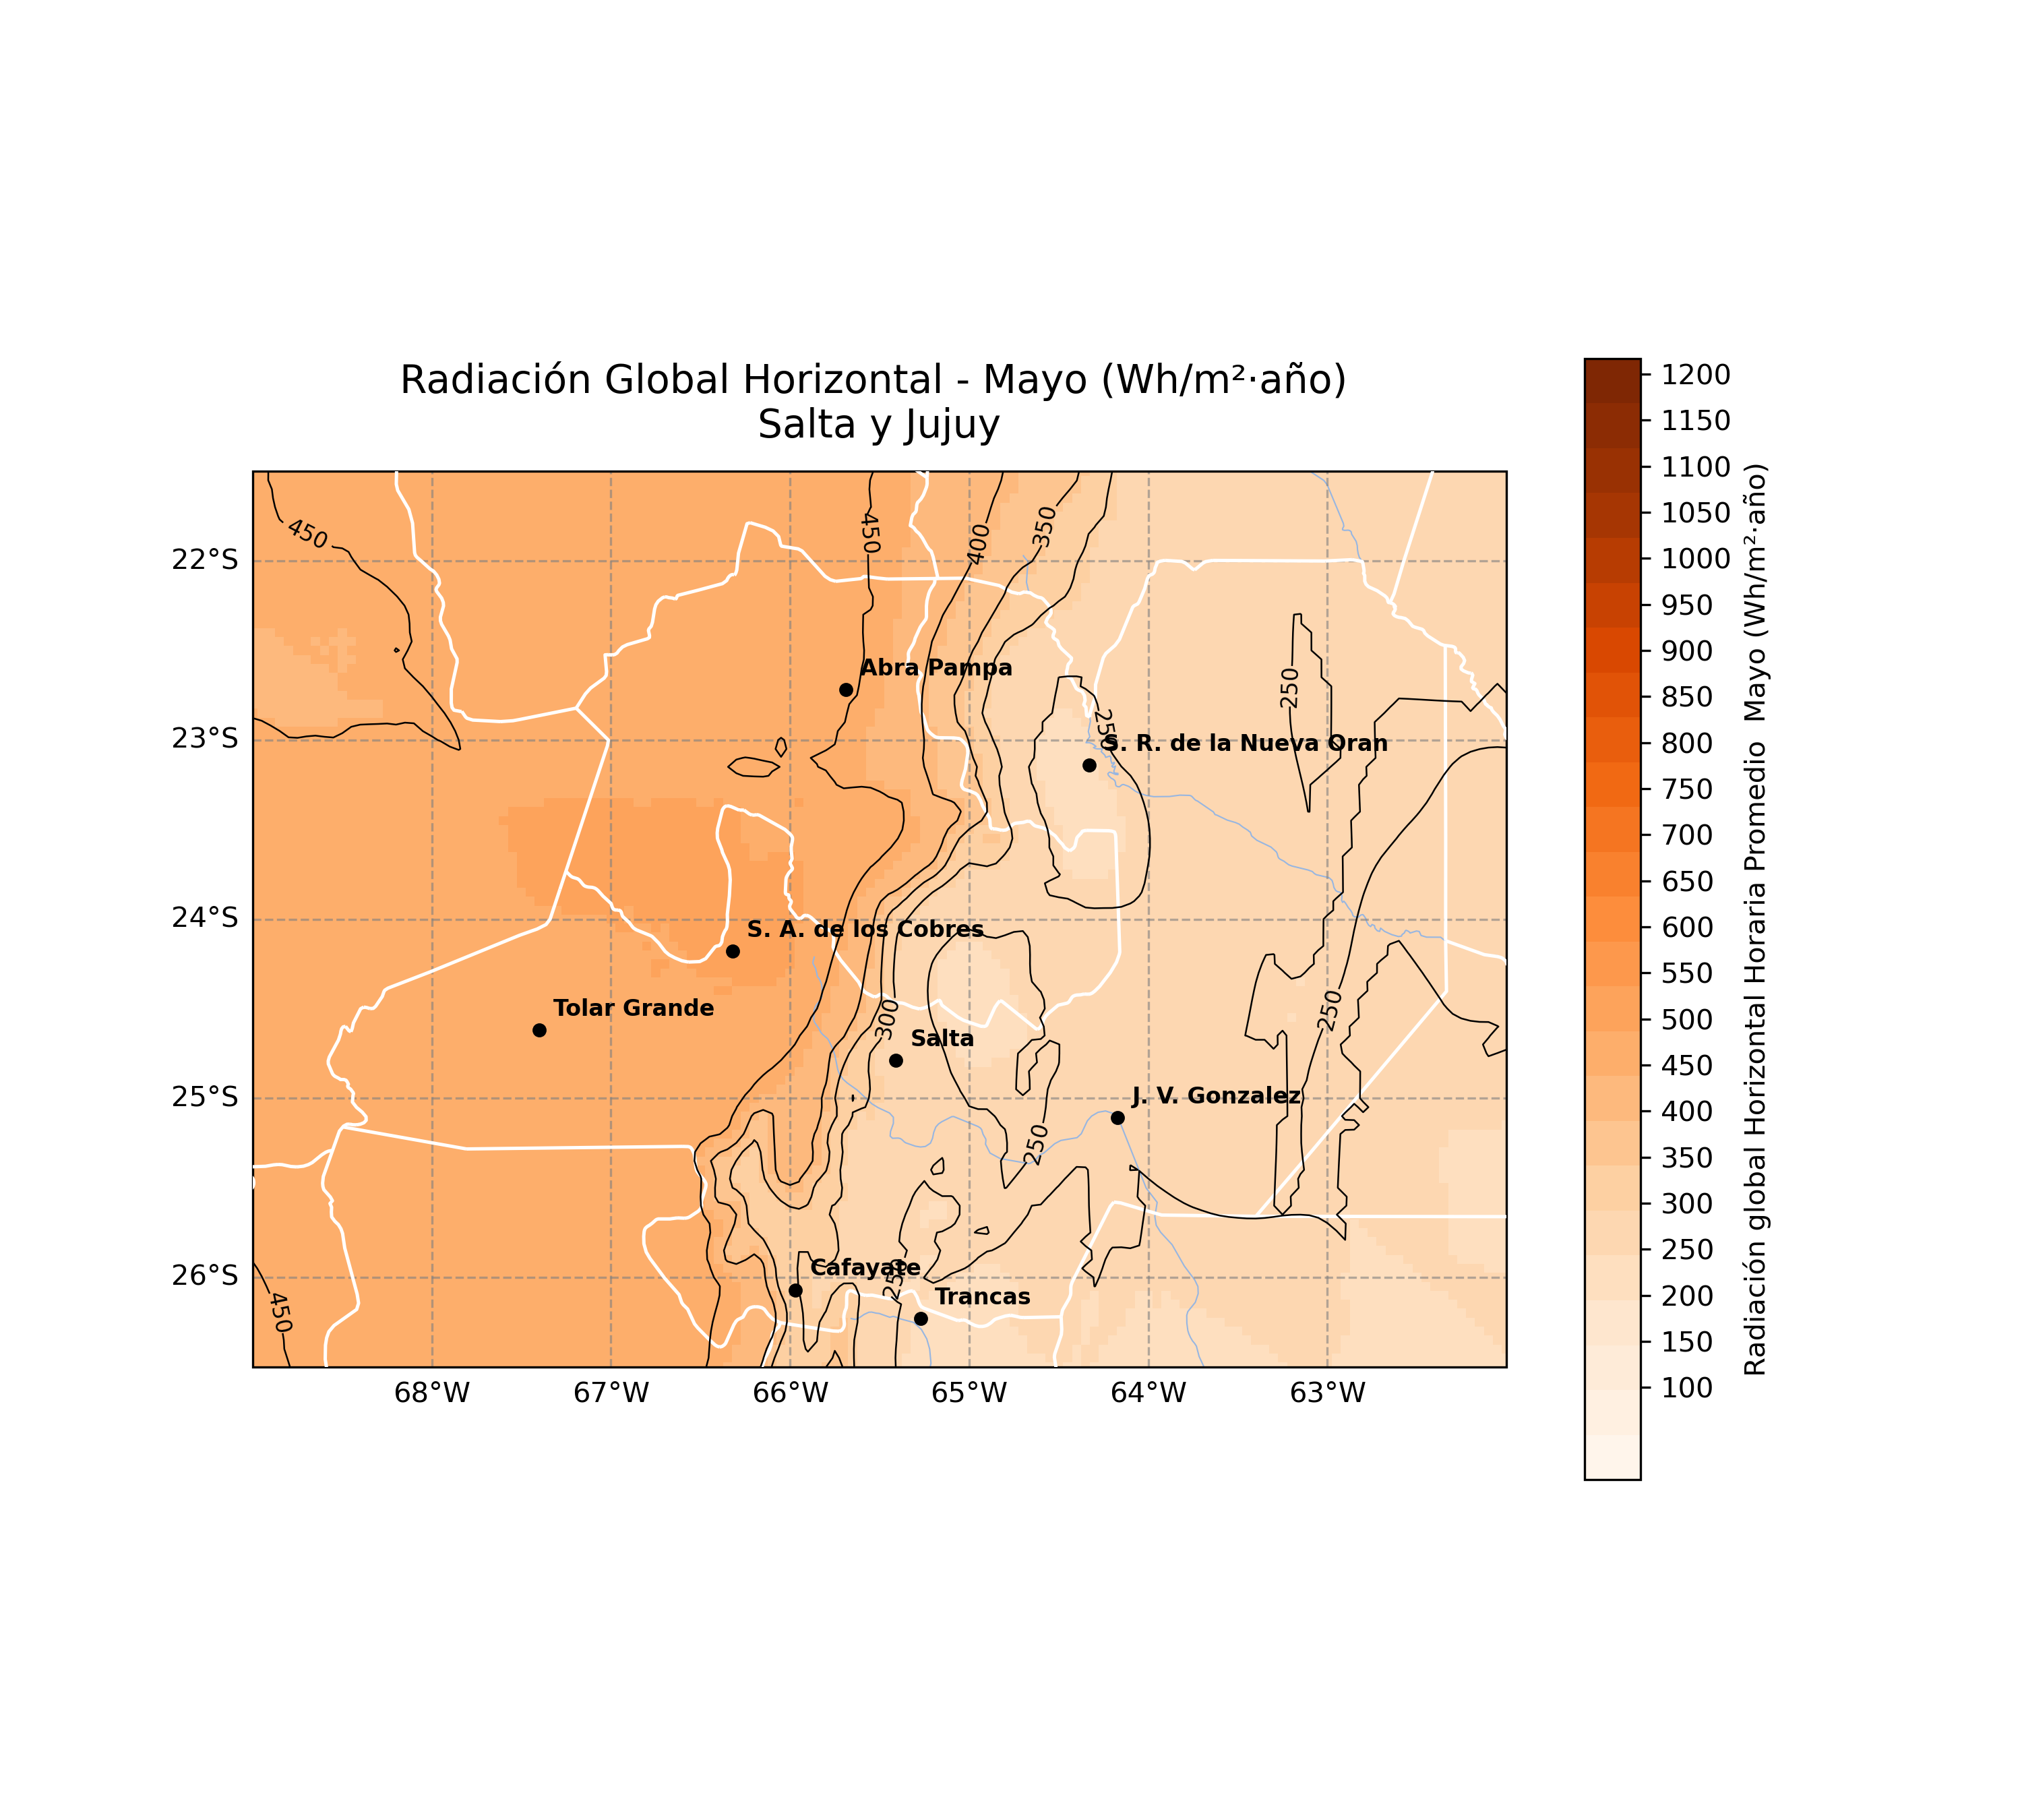
\includegraphics[width=0.95\textwidth]{figuras/Mapas/5_Mayo.png}
\caption{Mapa de GHI medio mensual – Mayo (TMY).}
\end{figure}

\begin{figure}[H]
\centering
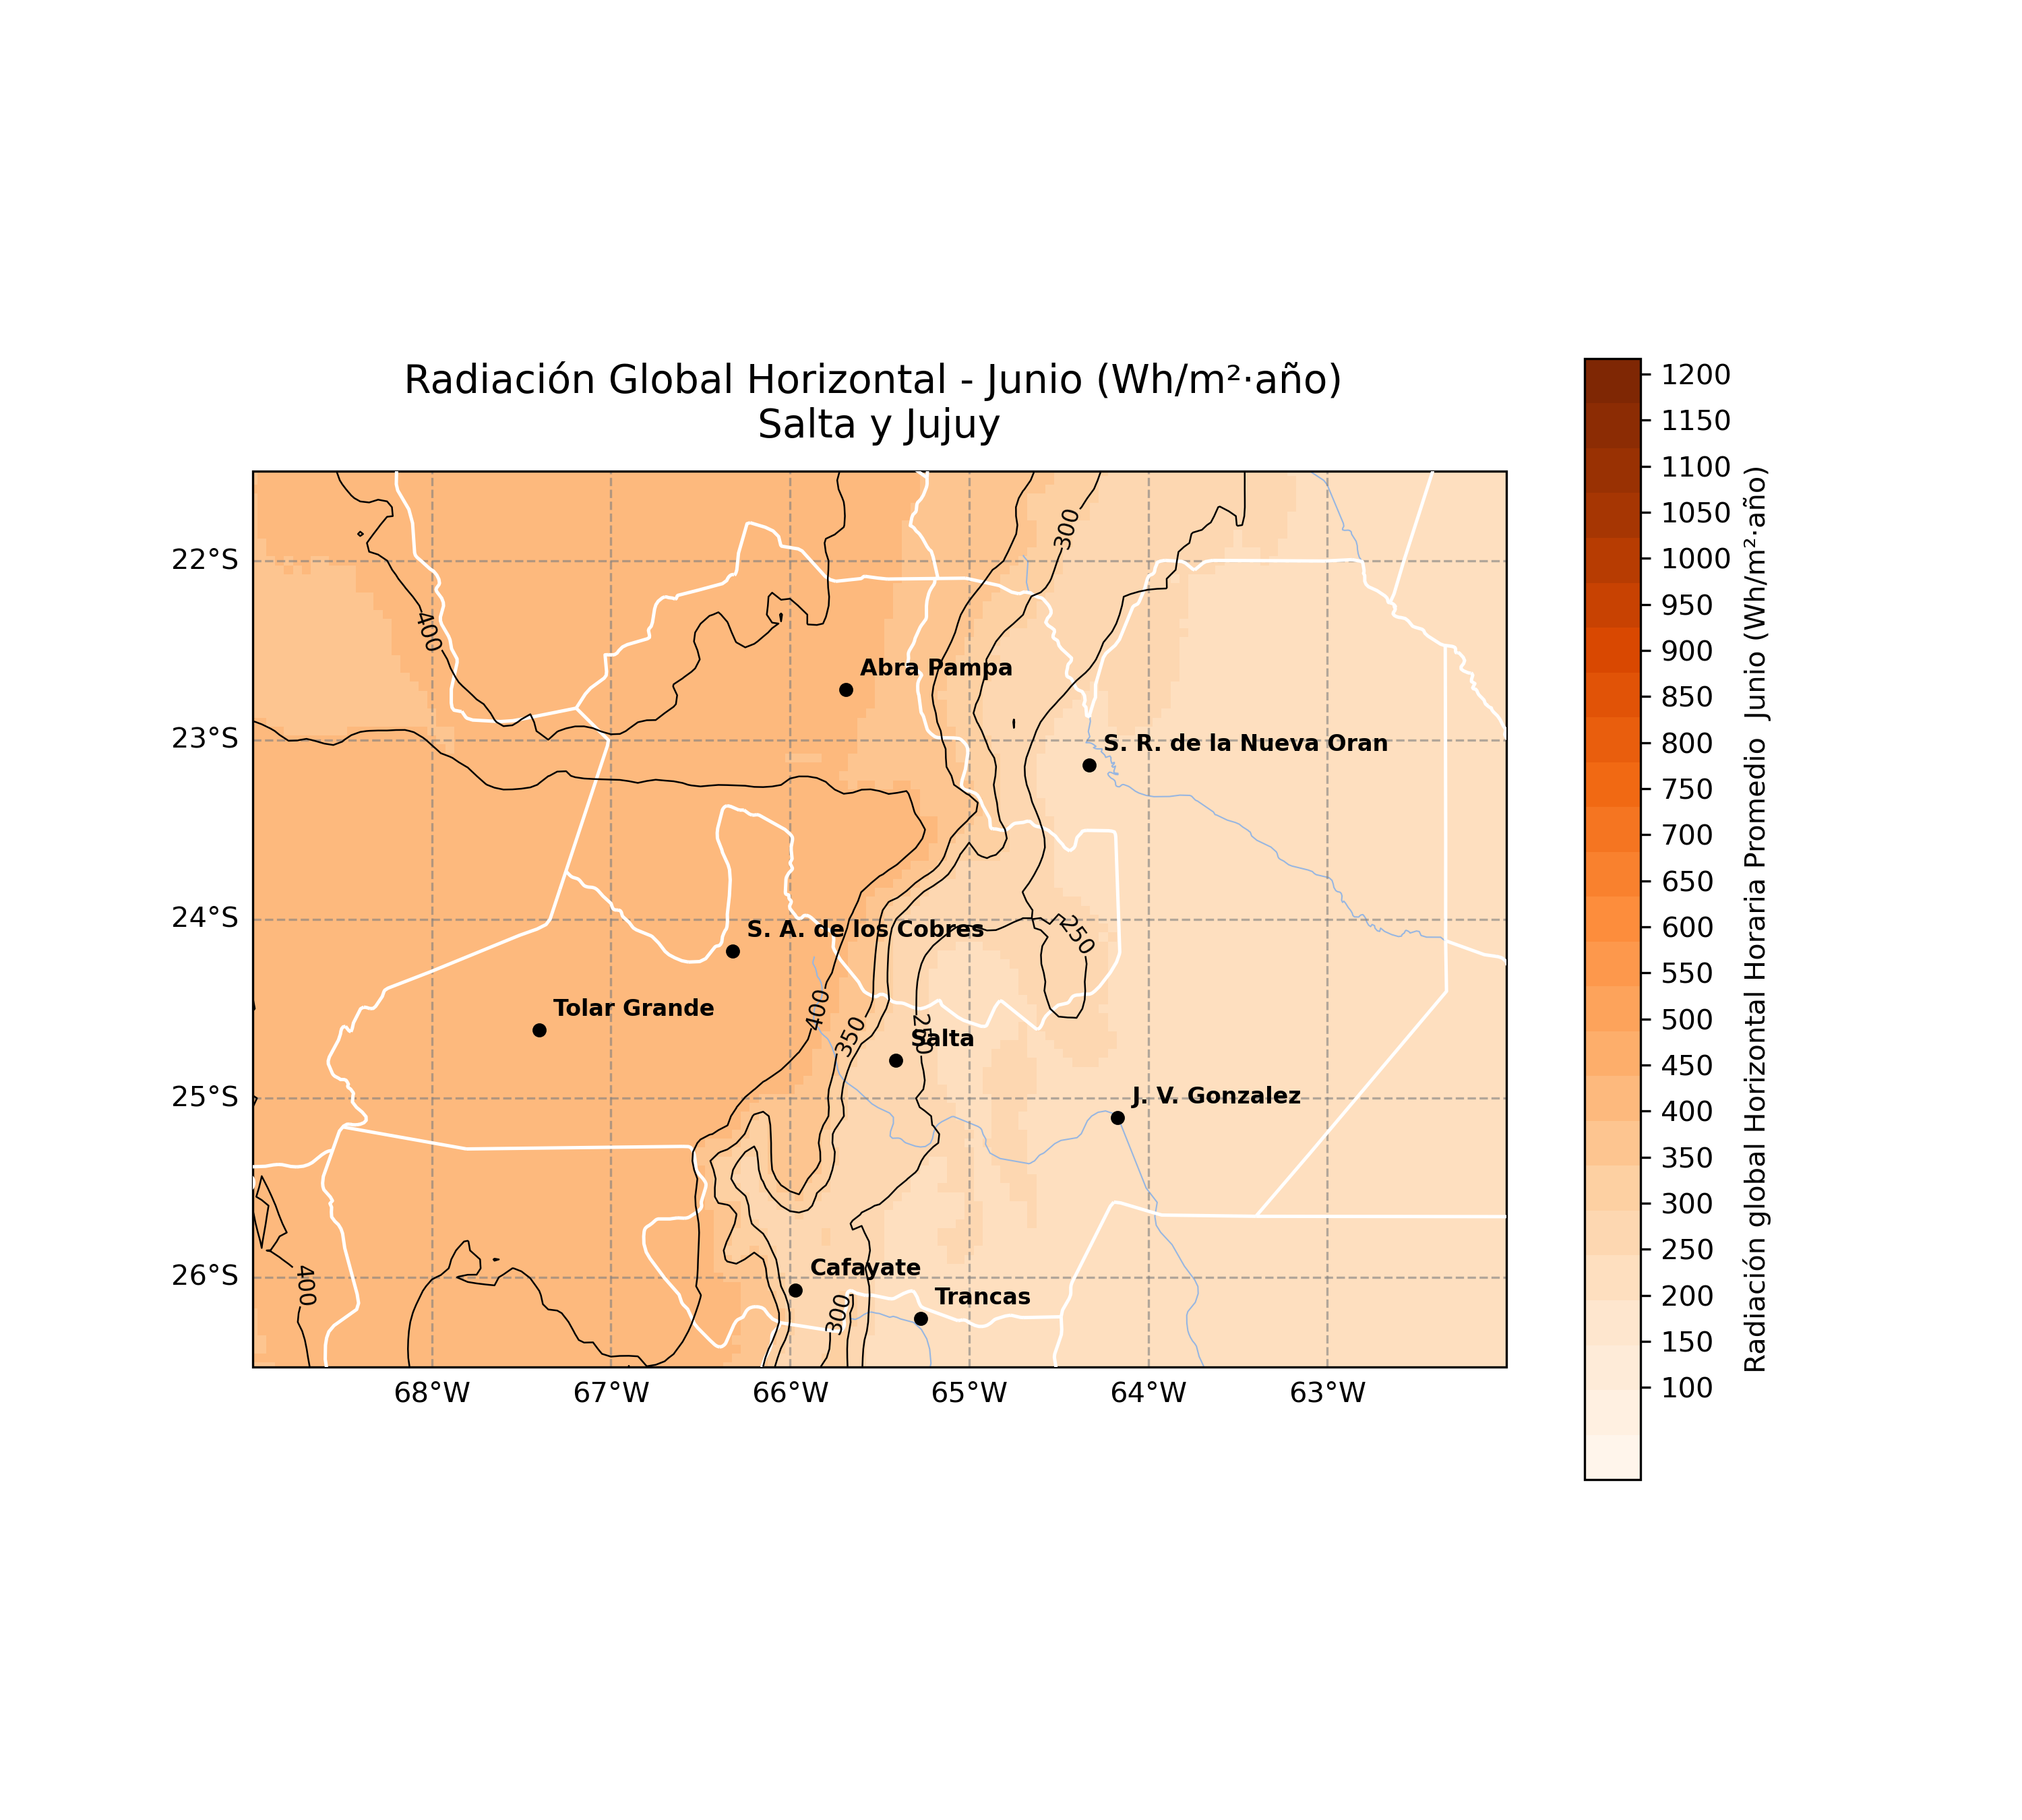
\includegraphics[width=0.95\textwidth]{figuras/Mapas/6_Junio.png}
\caption{Mapa de GHI medio mensual – Junio (TMY).}
\end{figure}

\begin{figure}[H]
\centering
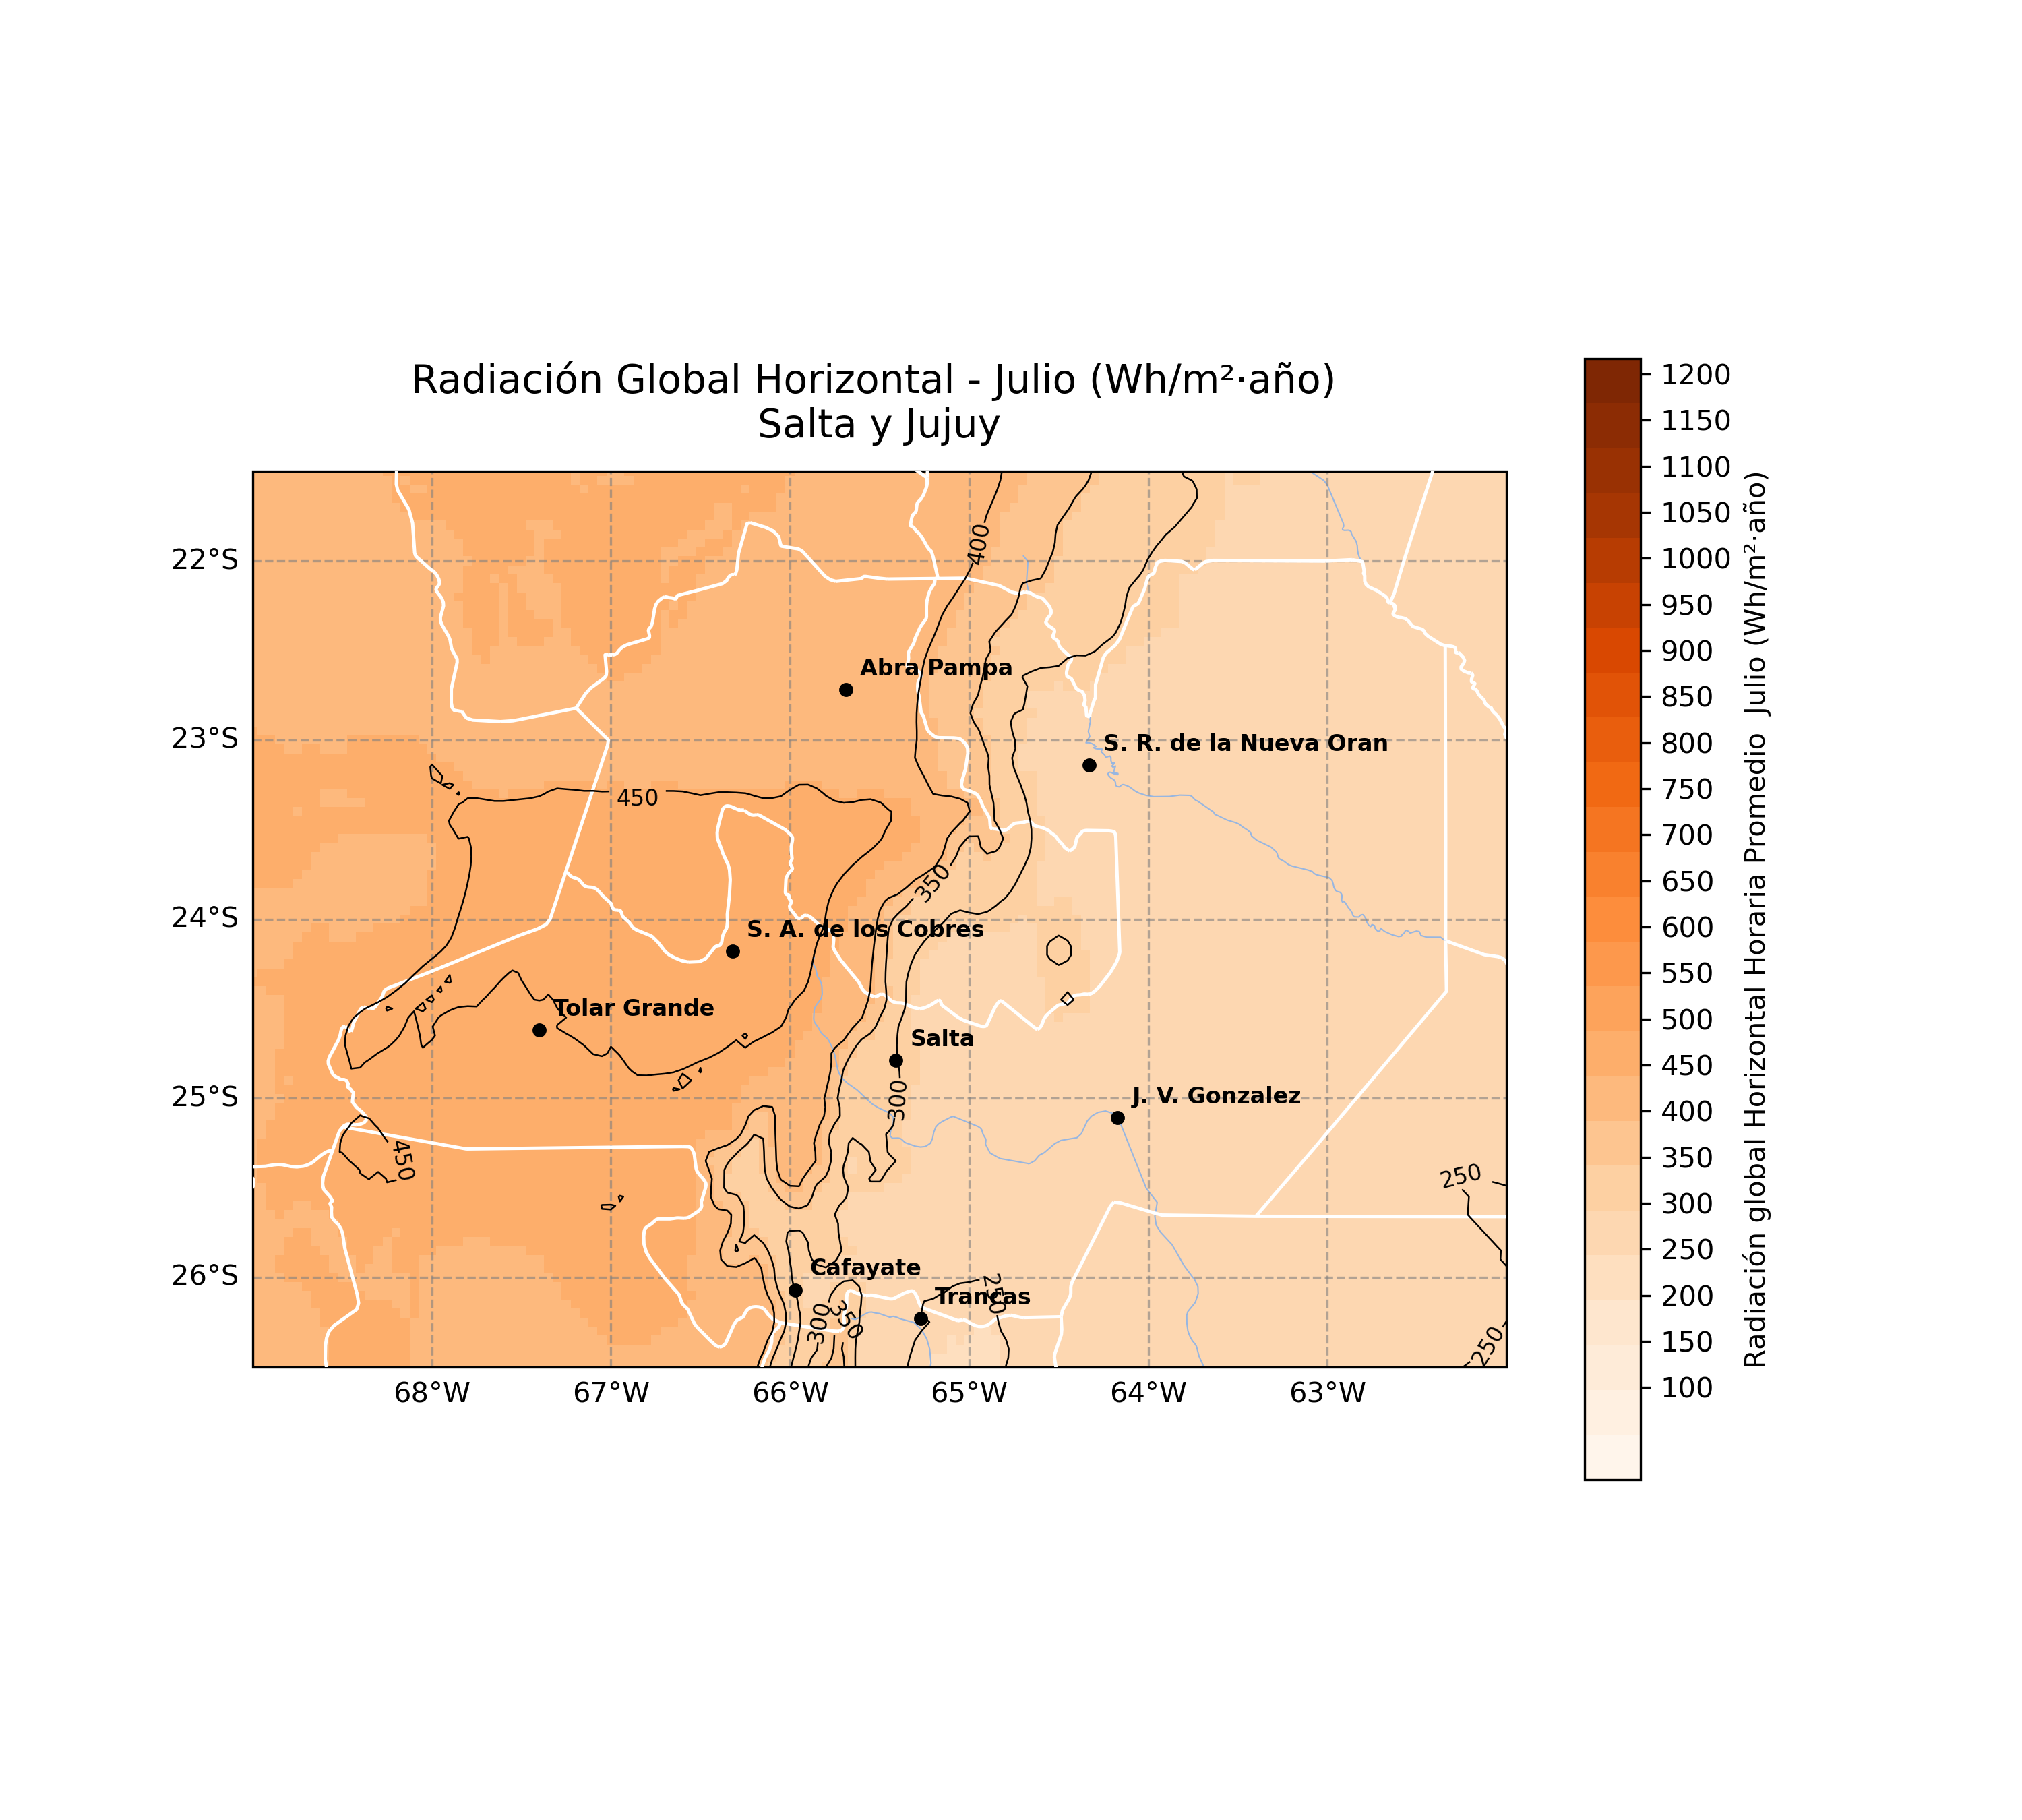
\includegraphics[width=0.95\textwidth]{figuras/Mapas/7_Julio.png}
\caption{Mapa de GHI medio mensual – Julio (TMY).}
\end{figure}

\begin{figure}[H]
\centering
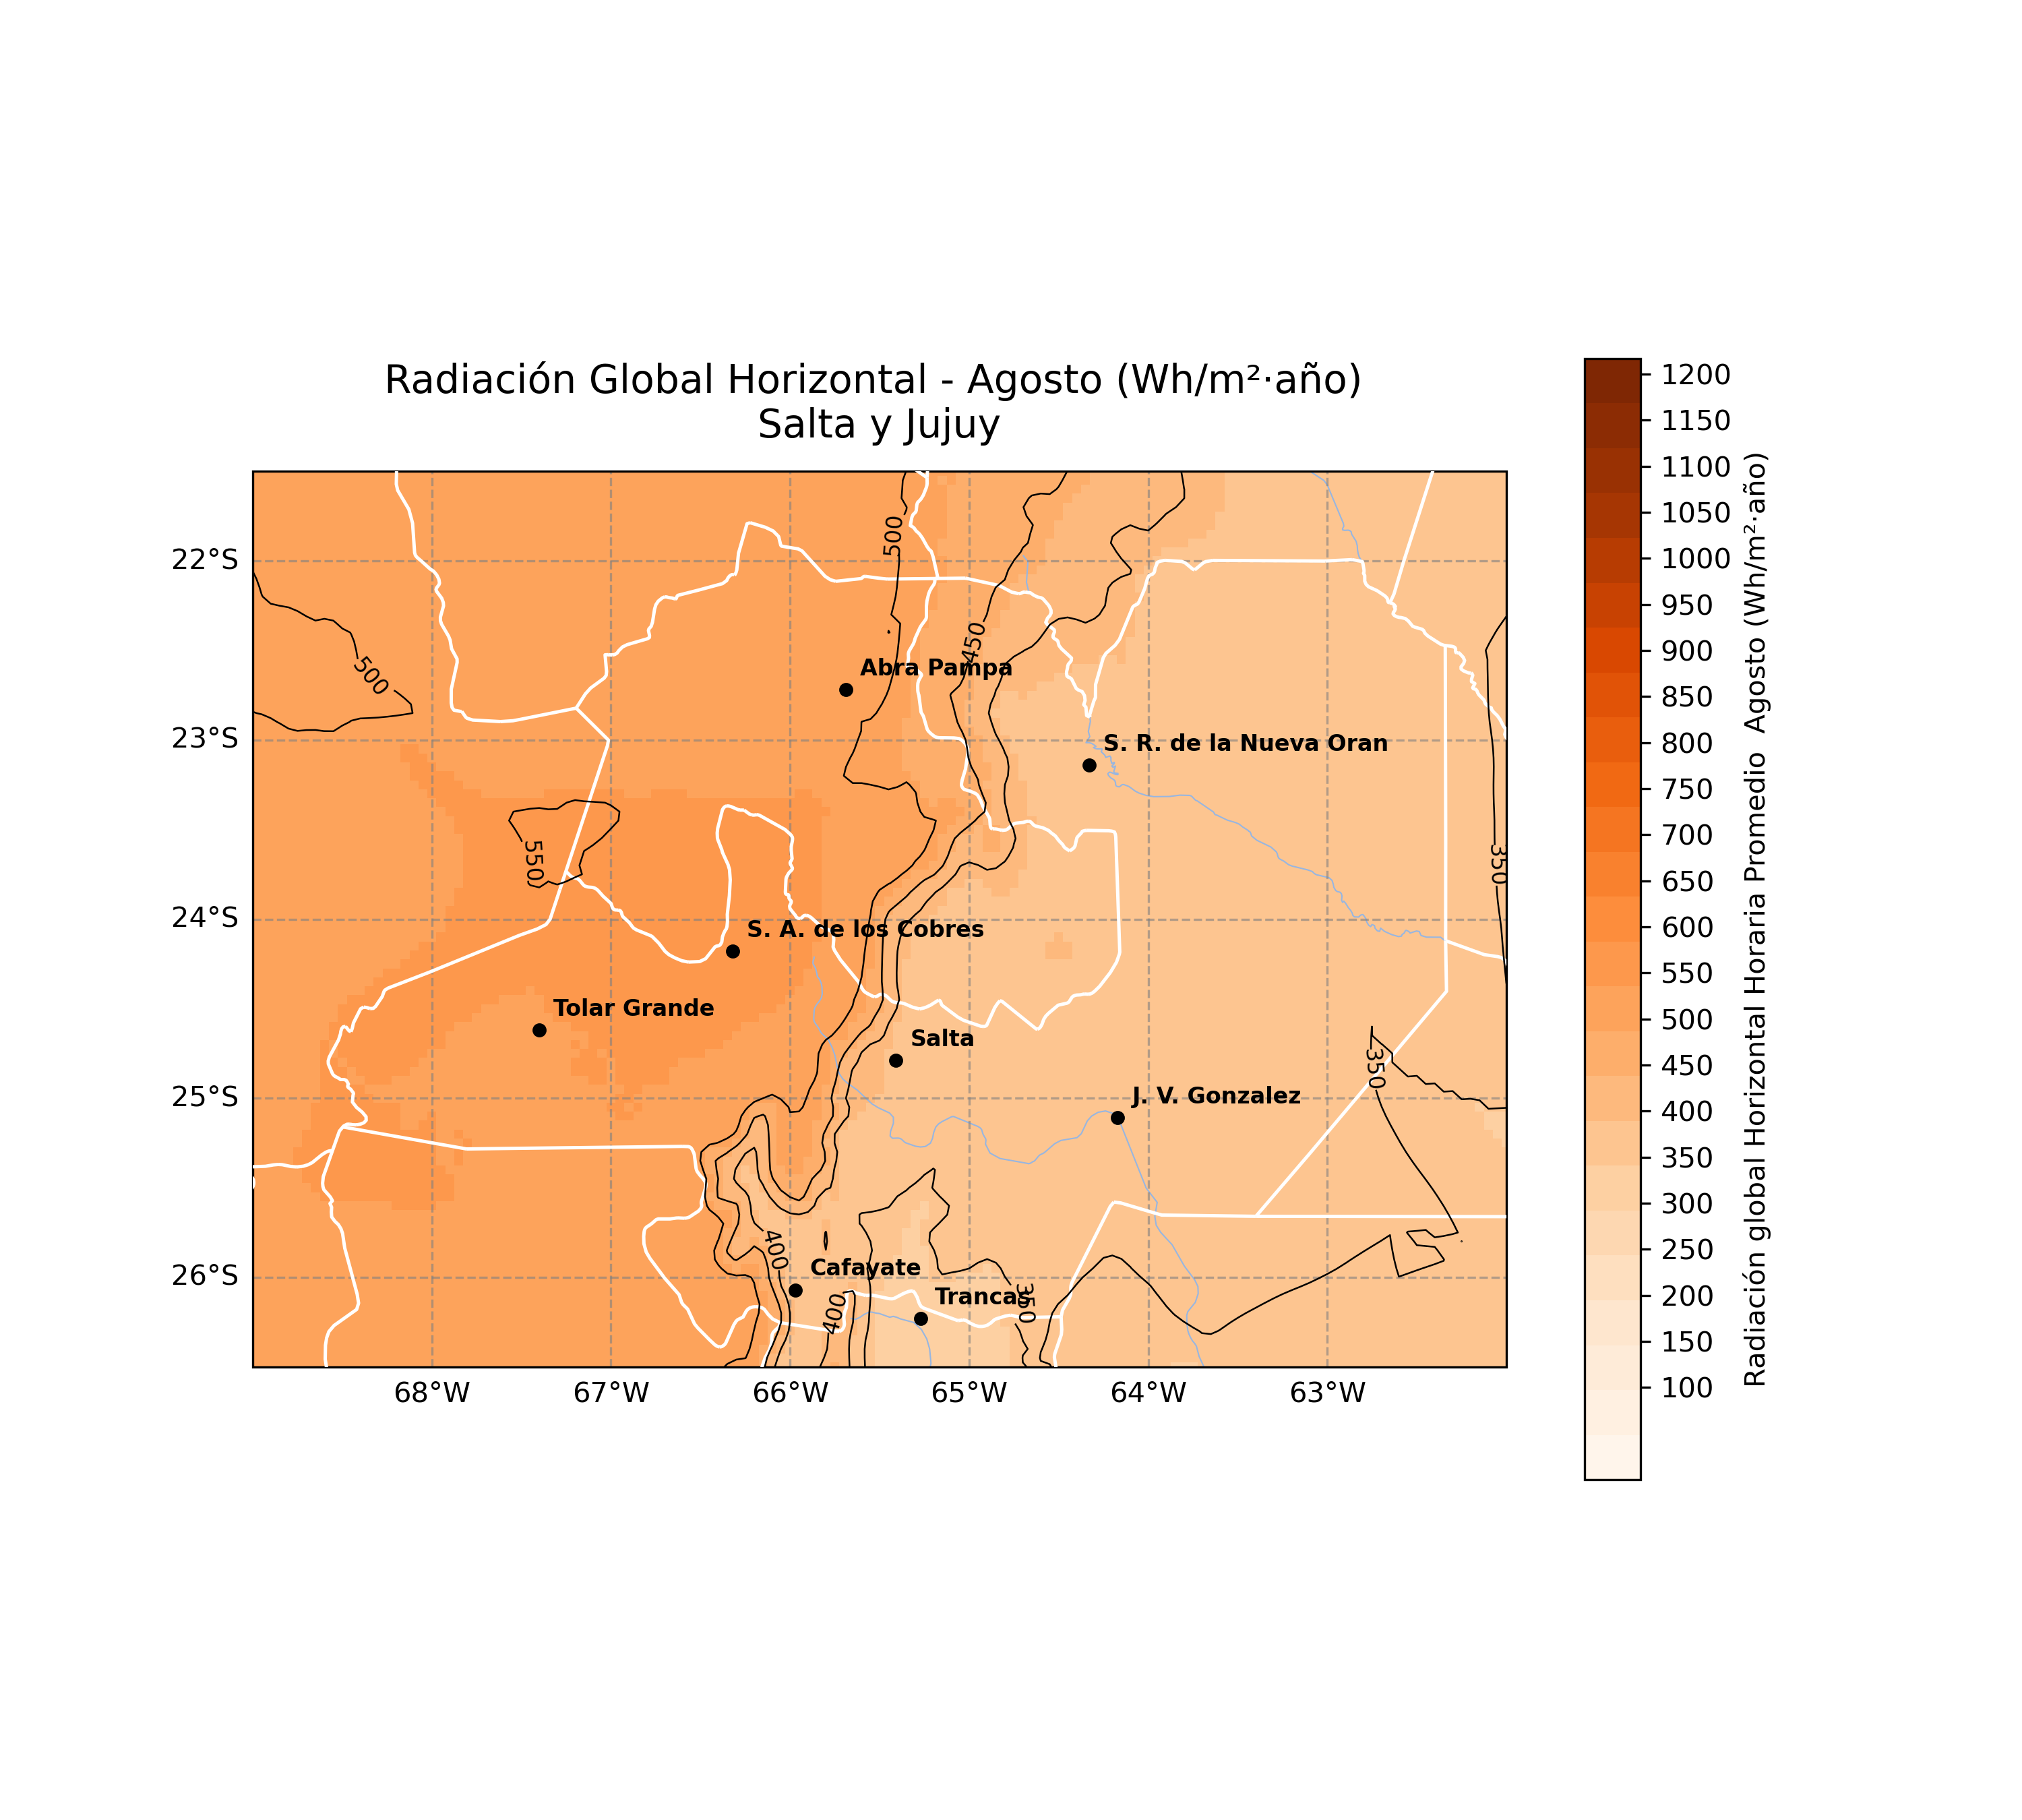
\includegraphics[width=0.95\textwidth]{figuras/Mapas/8_Agosto.png}
\caption{Mapa de GHI medio mensual – Agosto (TMY).}
\end{figure}

\begin{figure}[H]
\centering
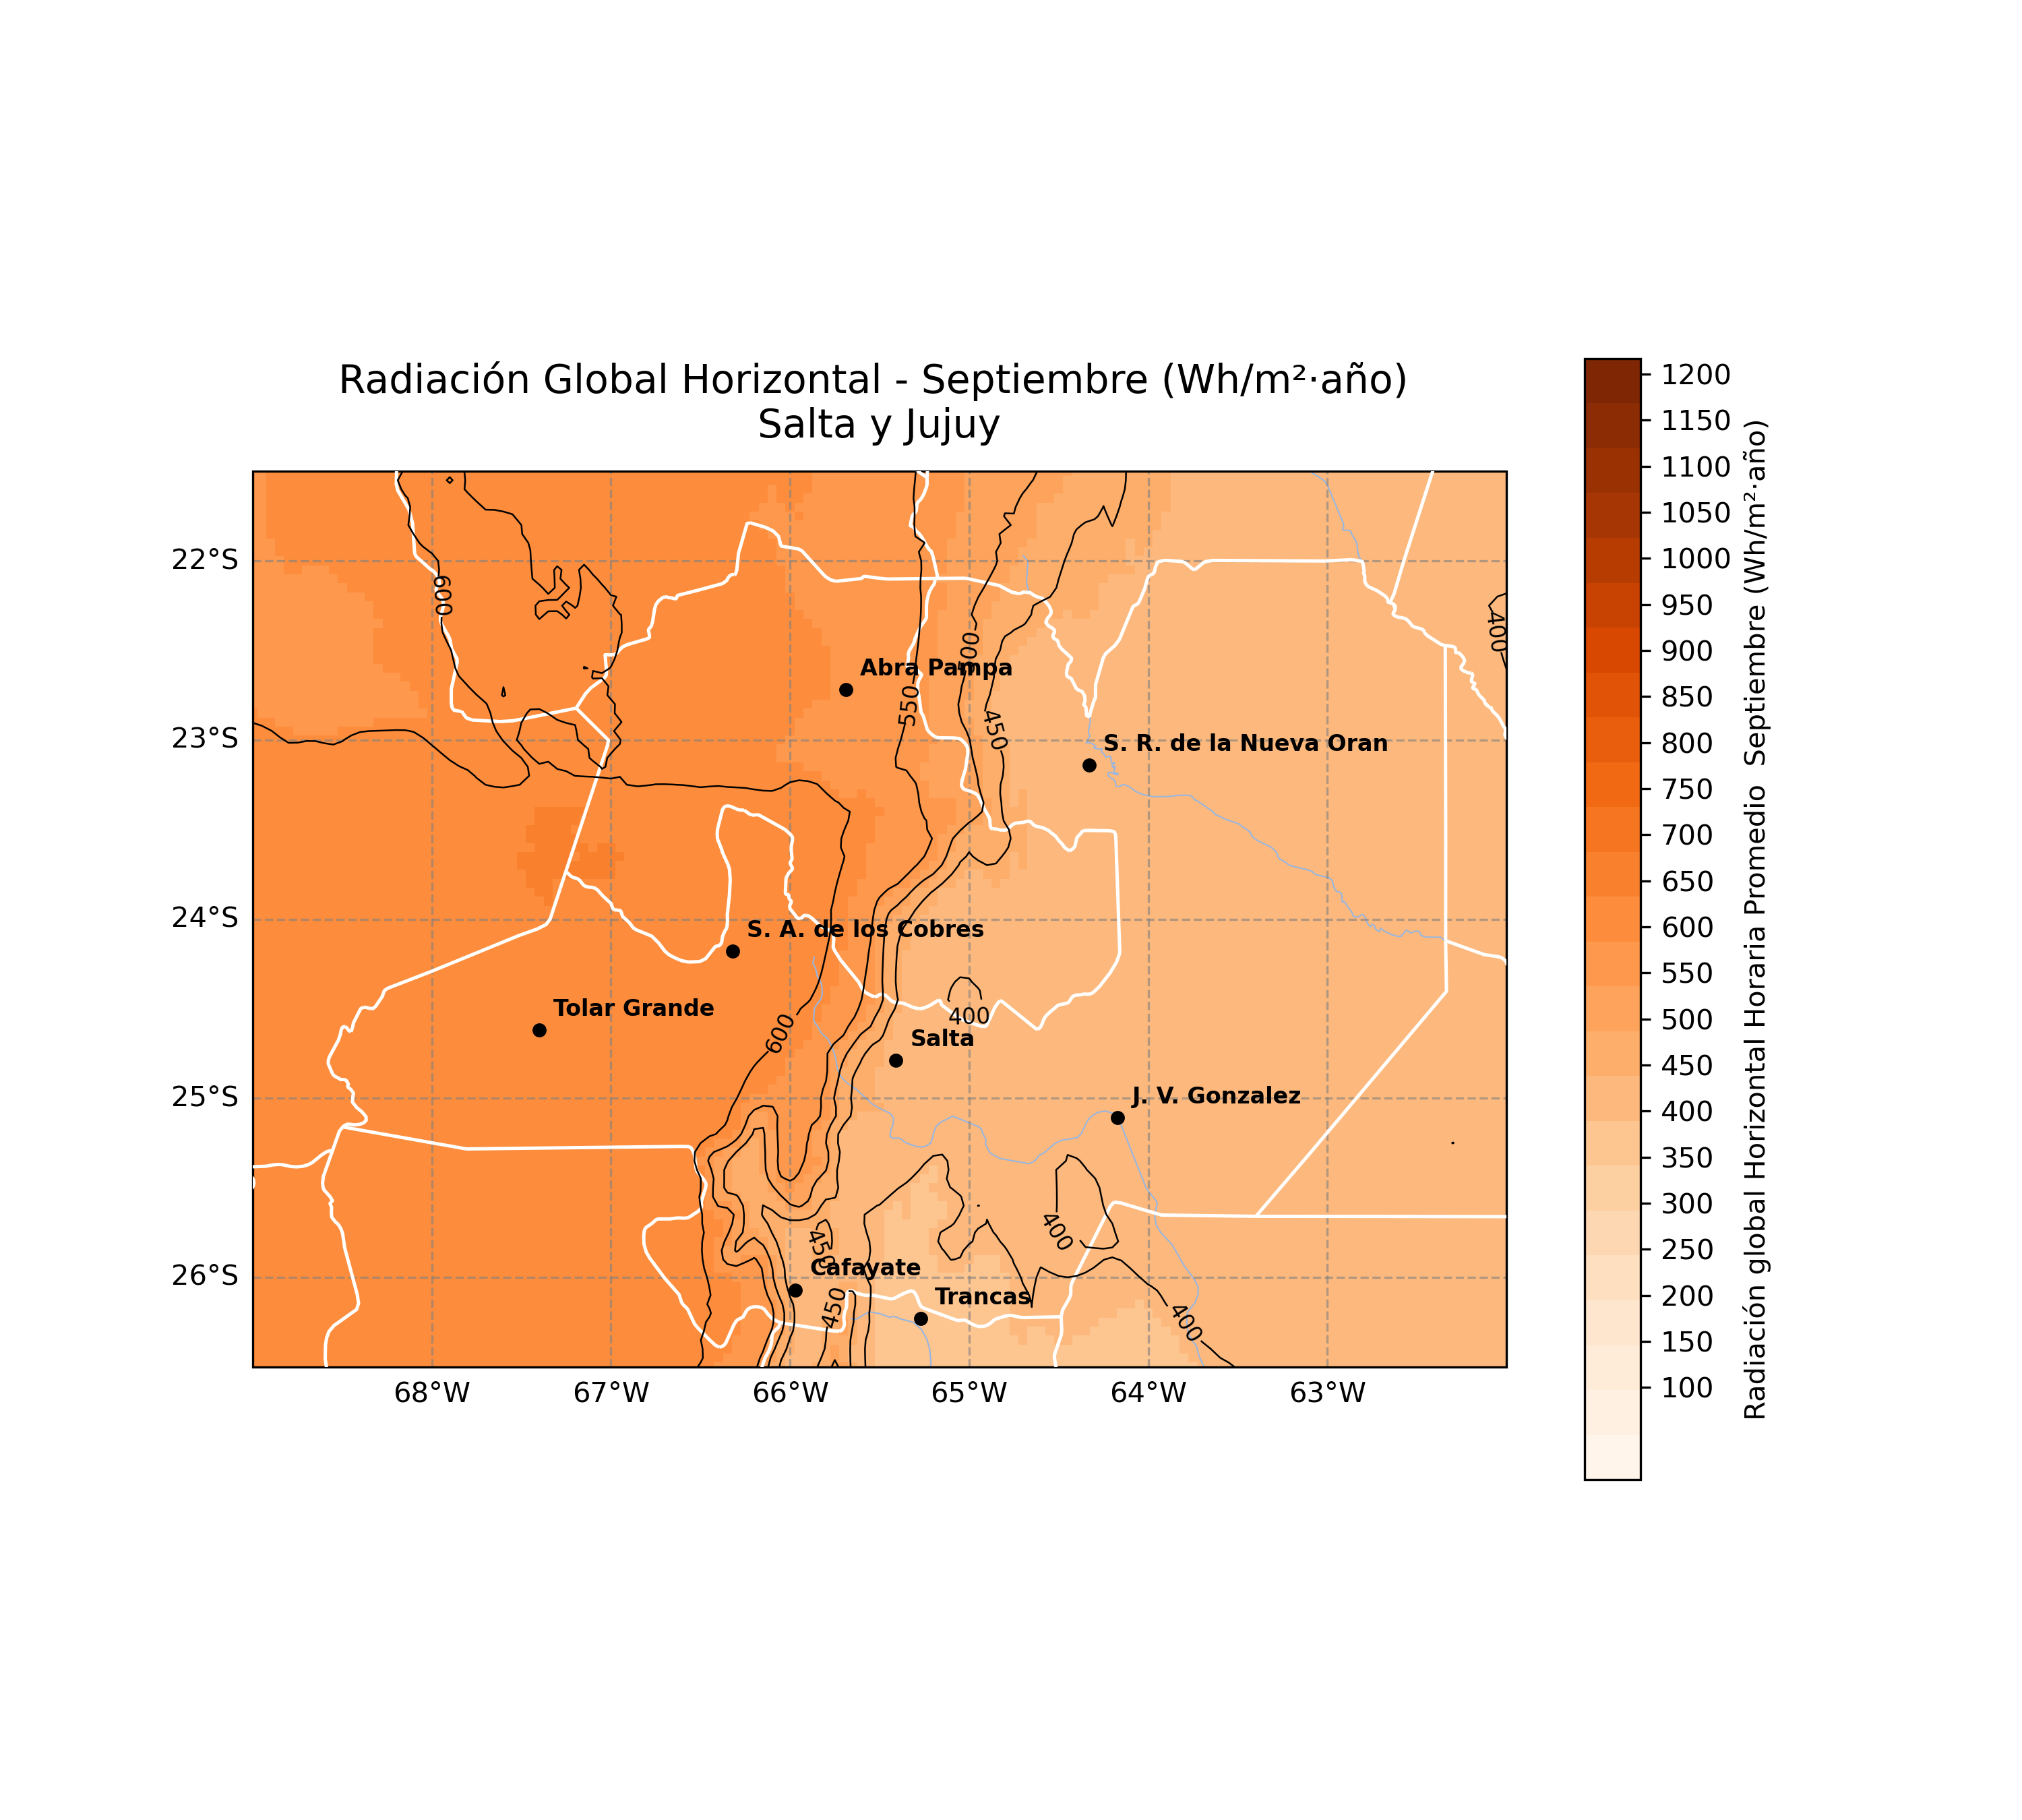
\includegraphics[width=0.95\textwidth]{figuras/Mapas/9_Septiembre.png}
\caption{Mapa de GHI medio mensual – Septiembre (TMY).}
\end{figure}

\begin{figure}[H]
\centering
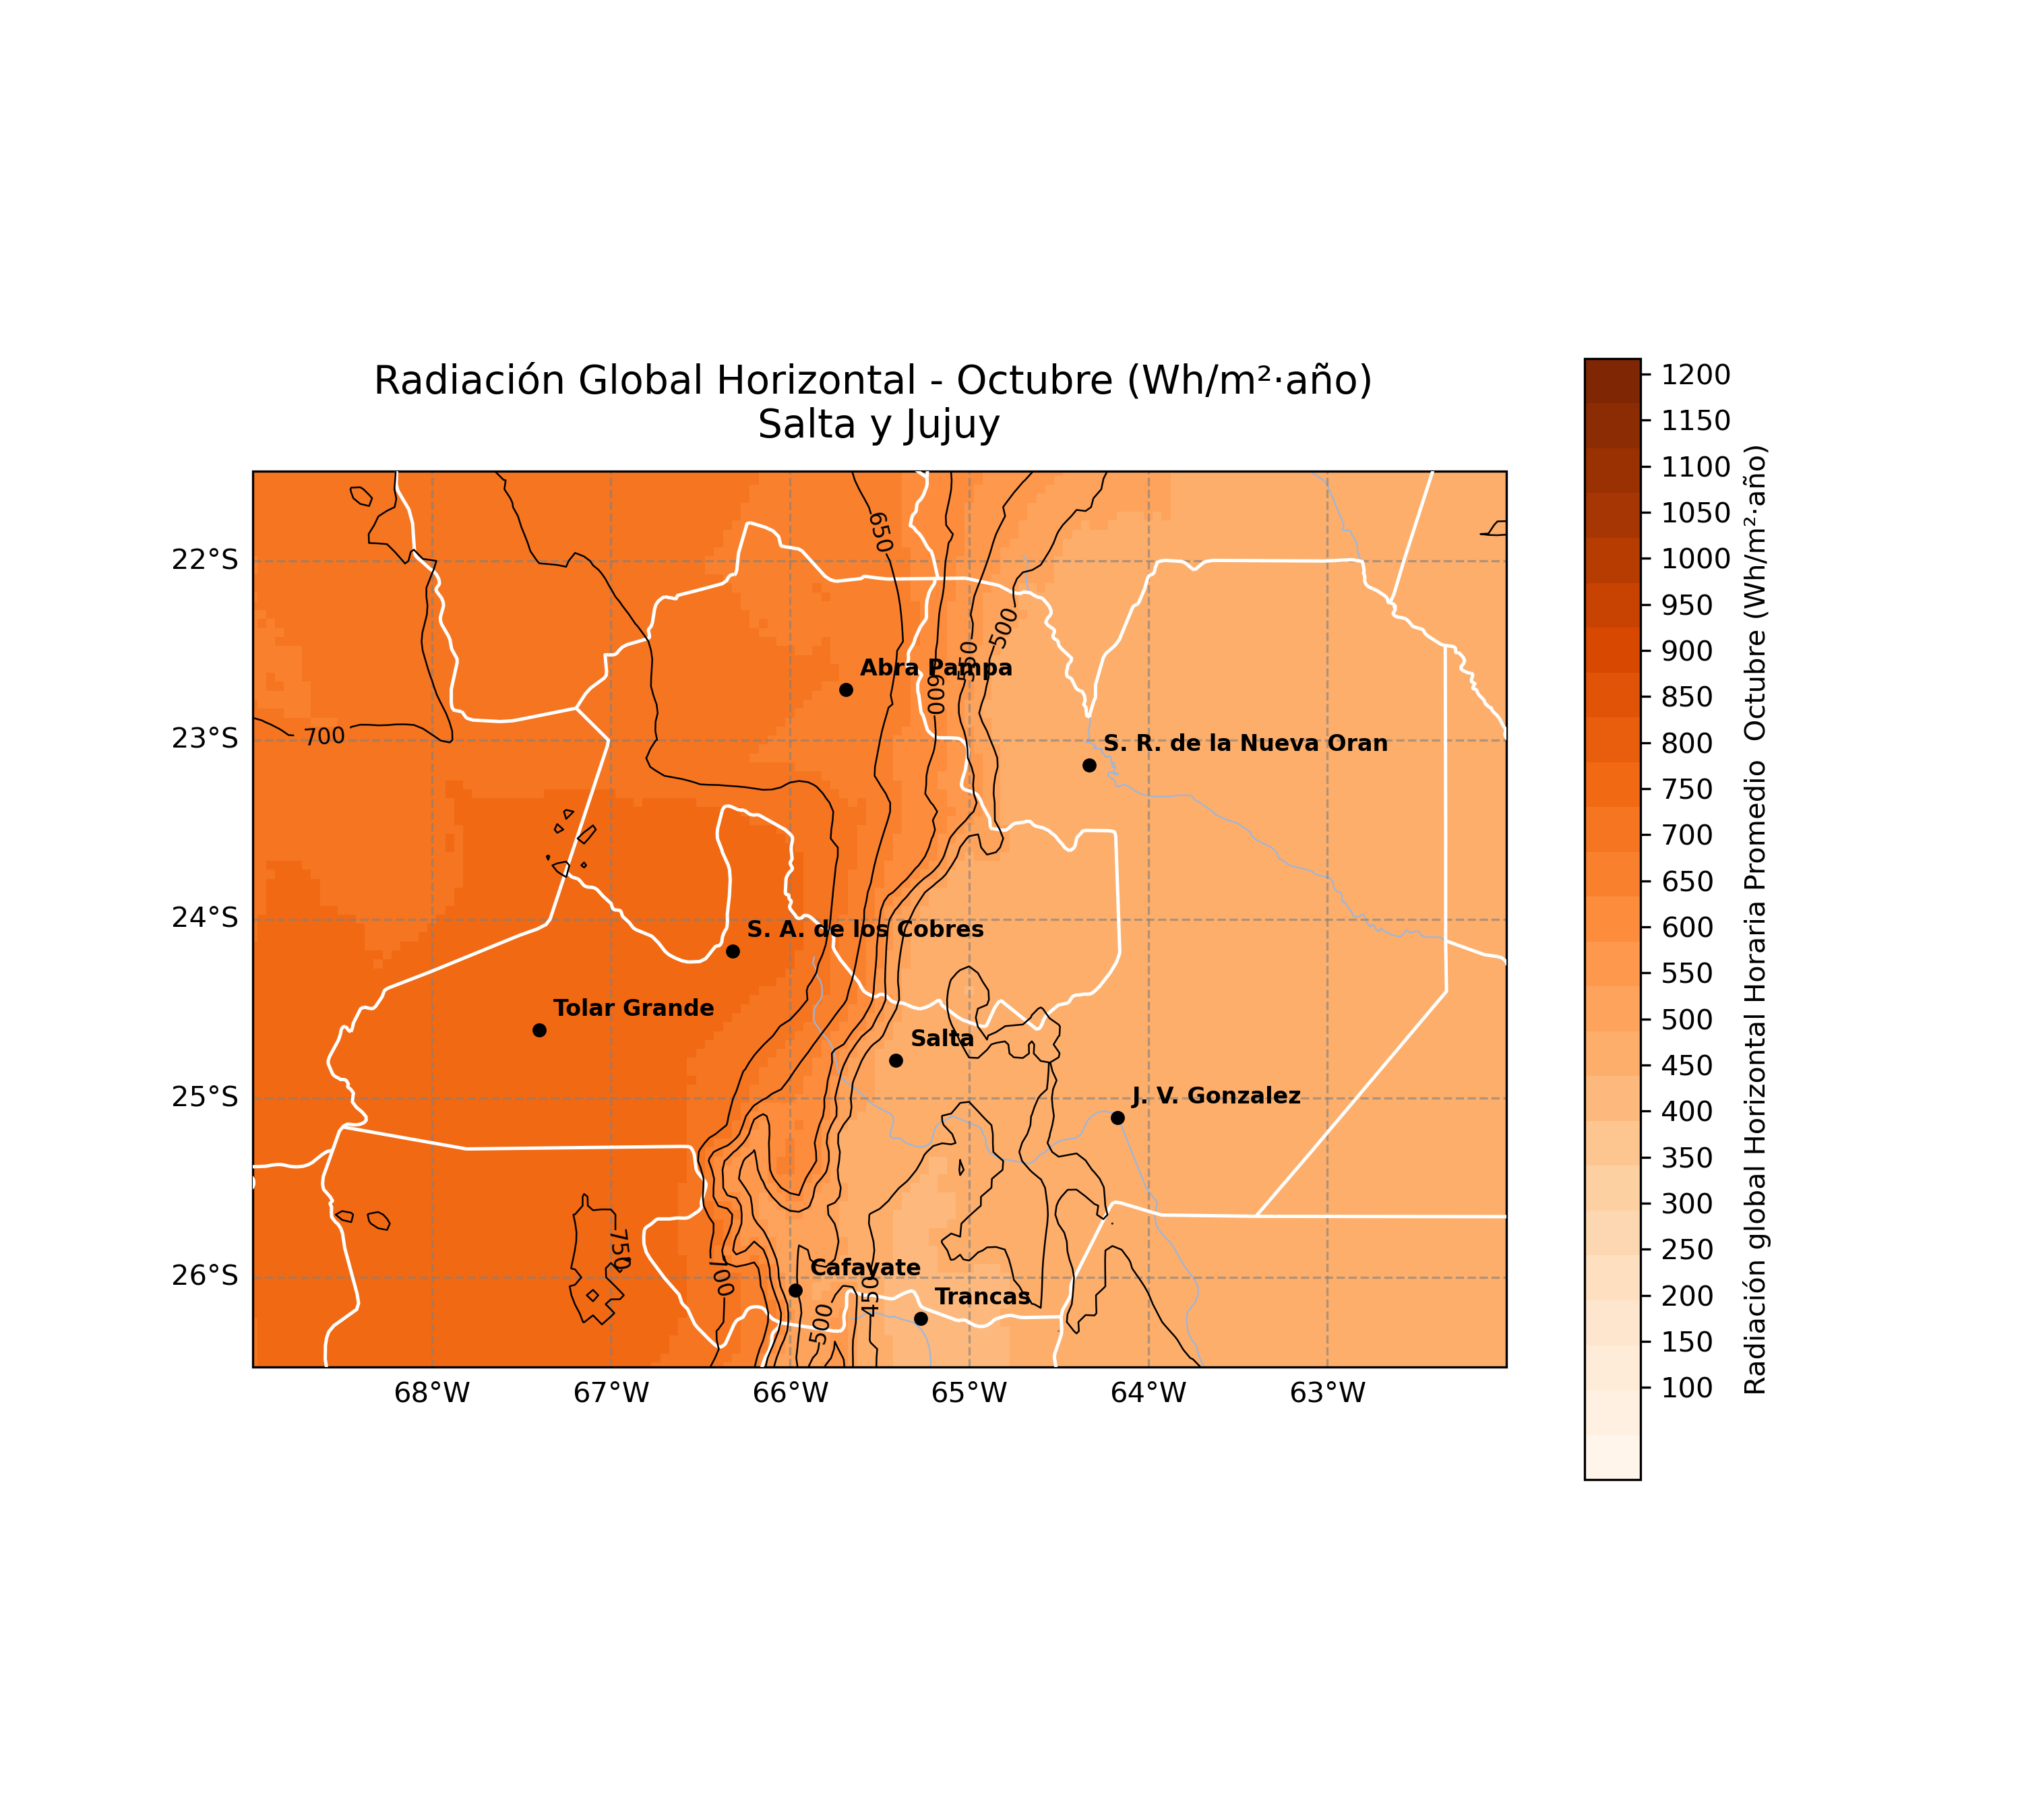
\includegraphics[width=0.95\textwidth]{figuras/Mapas/10_Octubre.png}
\caption{Mapa de GHI medio mensual – Octubre (TMY).}
\end{figure}

\begin{figure}[H]
\centering
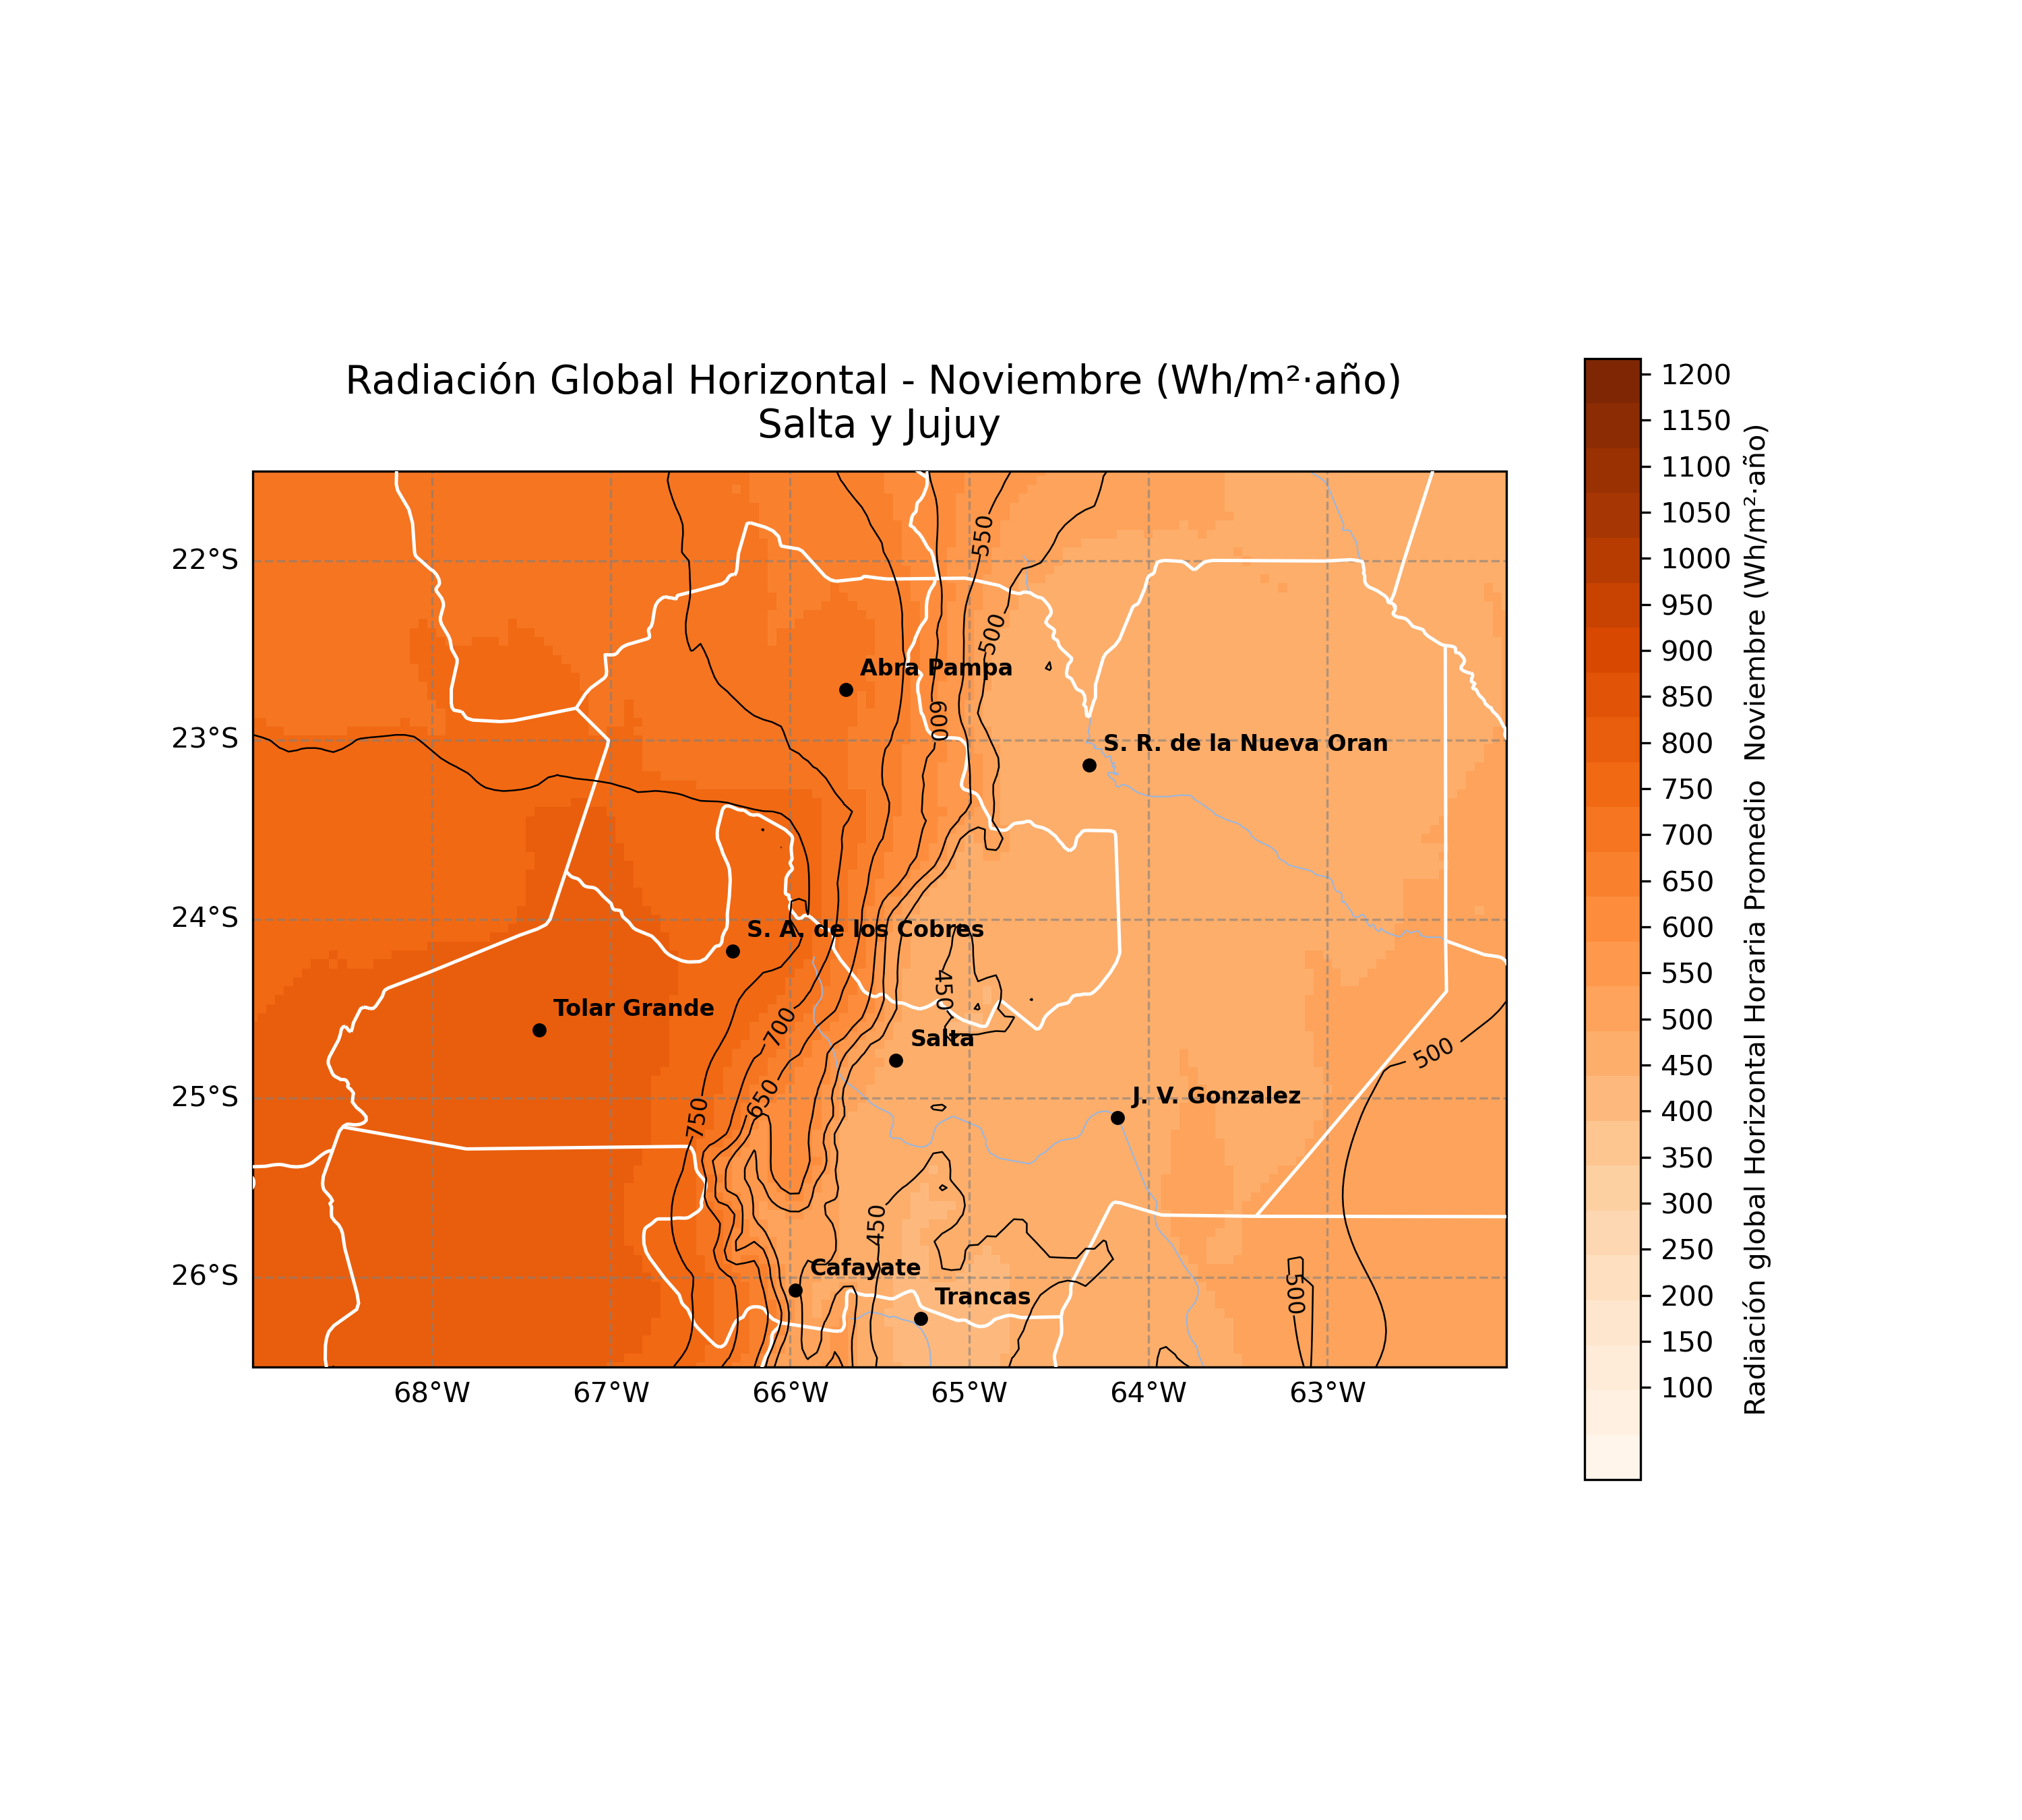
\includegraphics[width=0.95\textwidth]{figuras/Mapas/11_Noviembre.png}
\caption{Mapa de GHI medio mensual – Noviembre (TMY).}
\end{figure}

\begin{figure}[H]
\centering
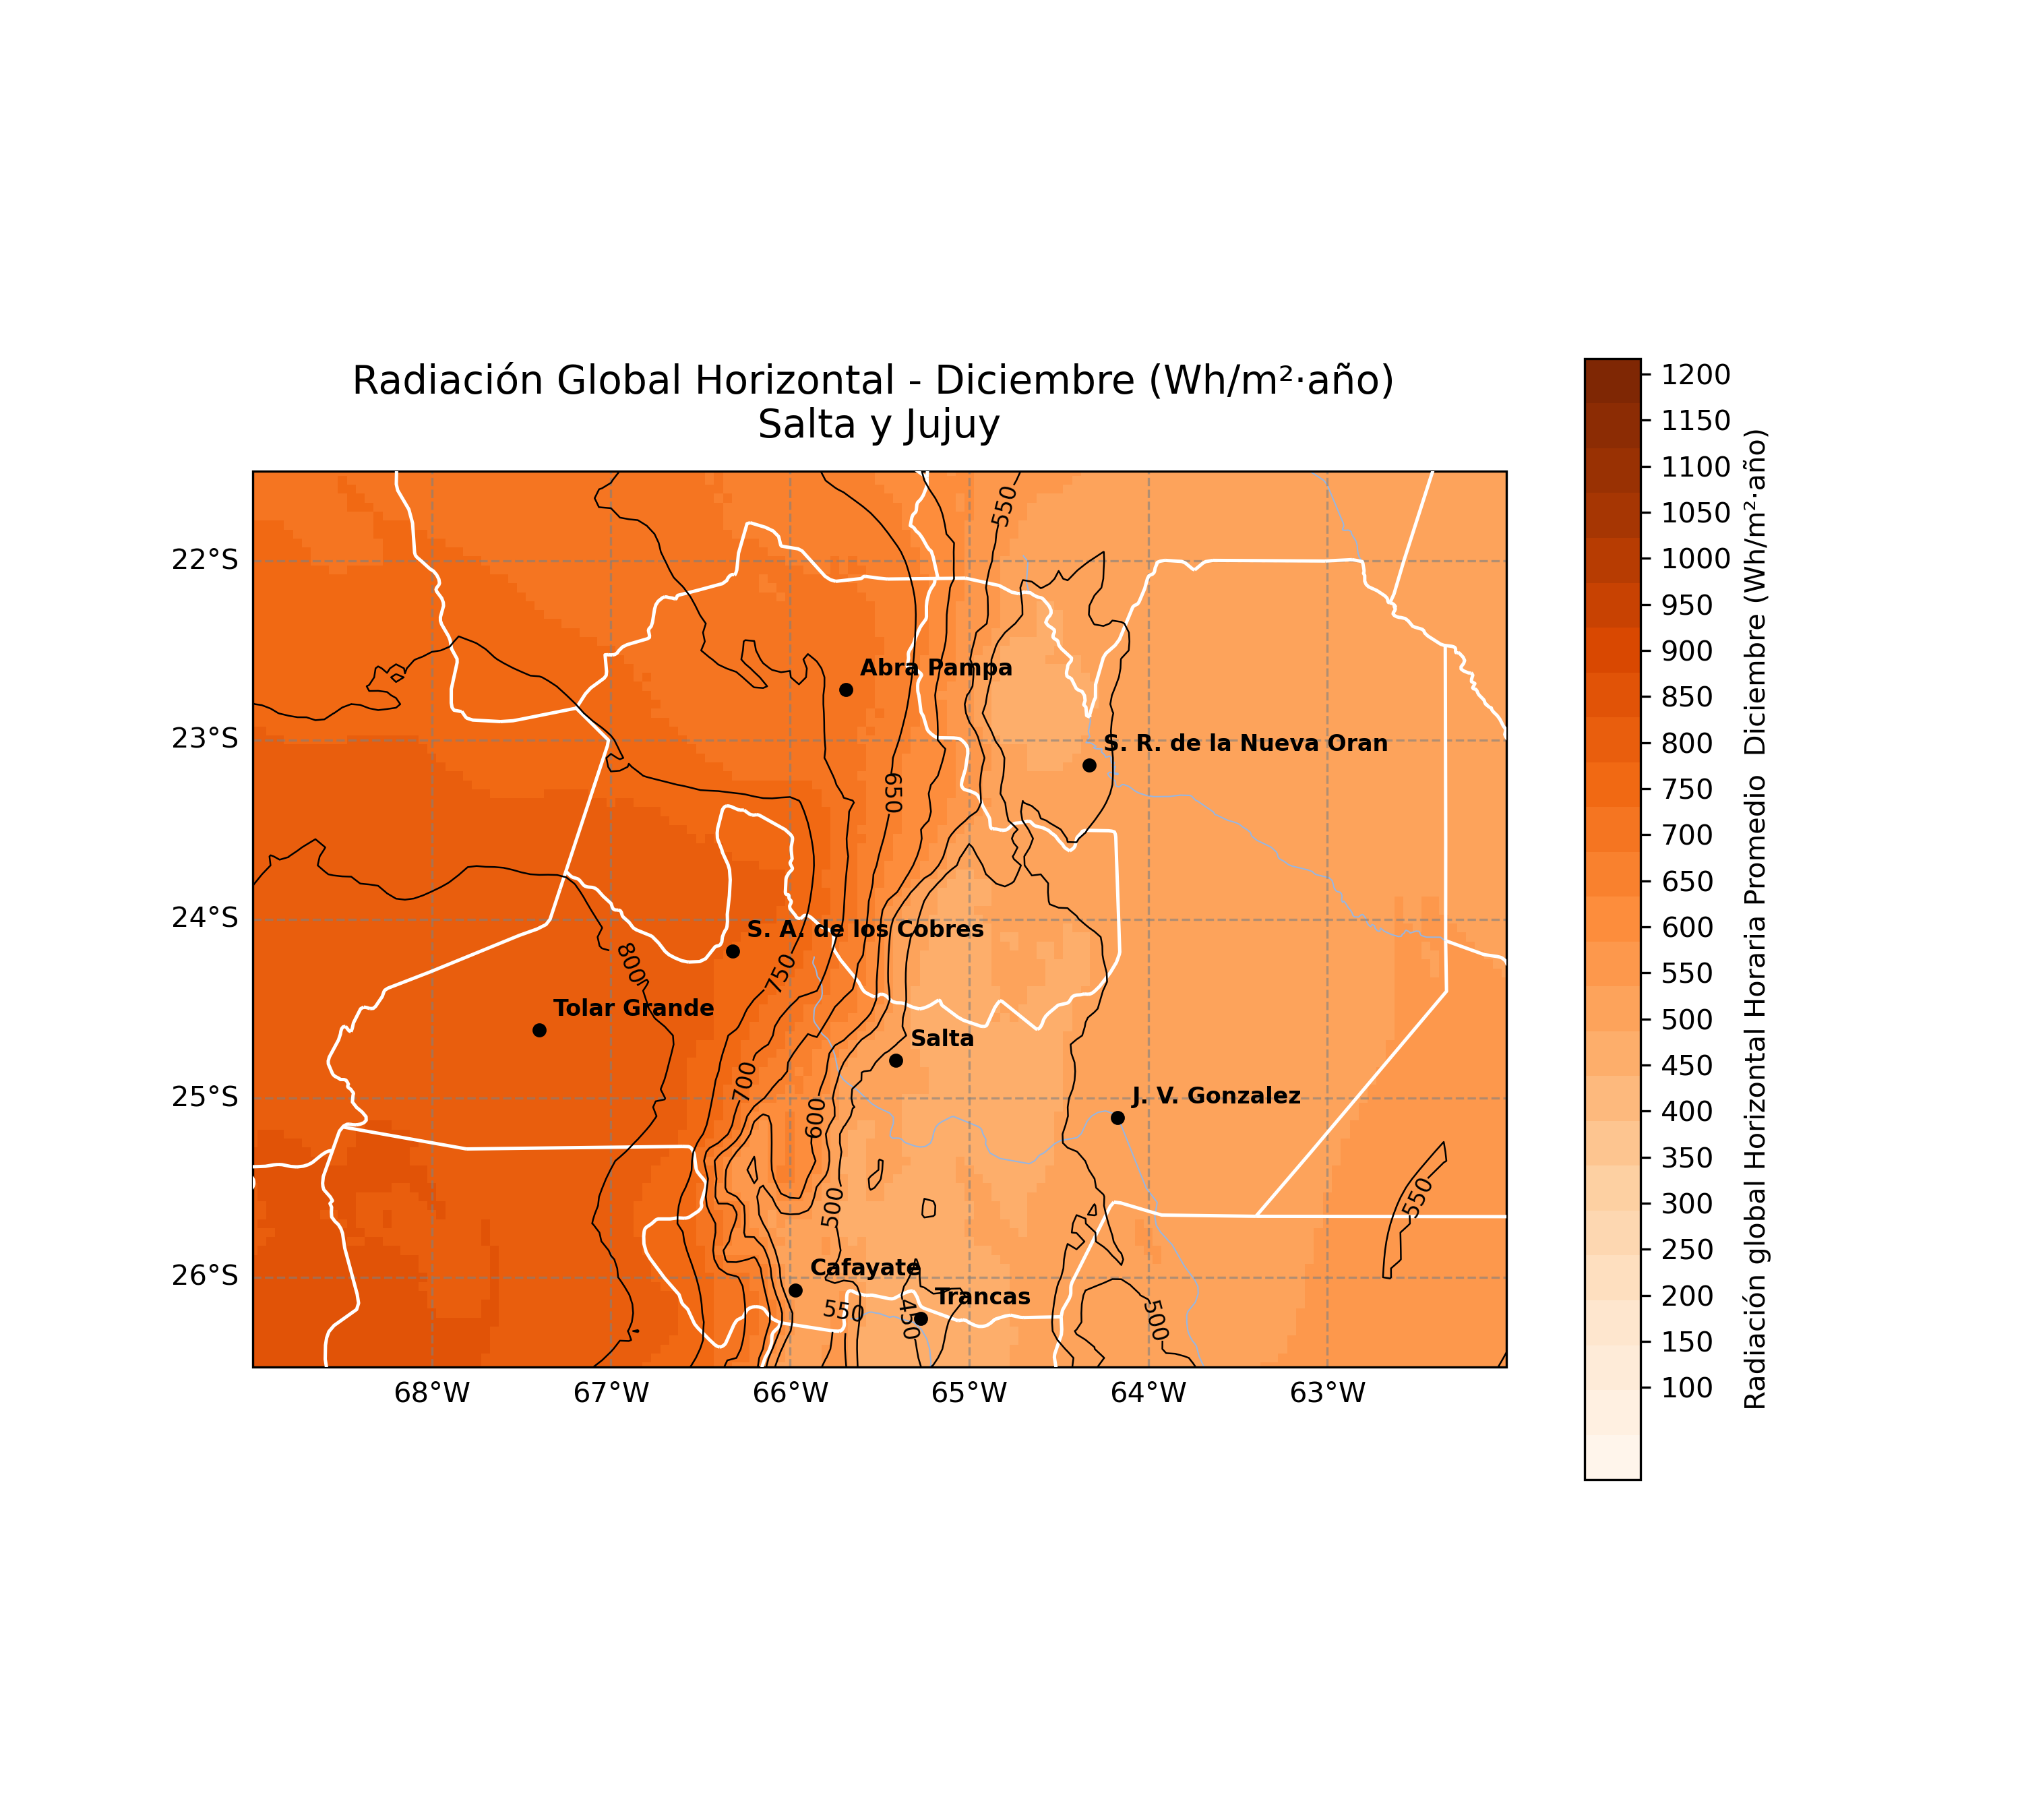
\includegraphics[width=0.95\textwidth]{figuras/Mapas/12_Diciembre.png}
\caption{Mapa de GHI medio mensual – Diciembre (TMY).}
\end{figure}




	
\begin{figure}
    \centering	
        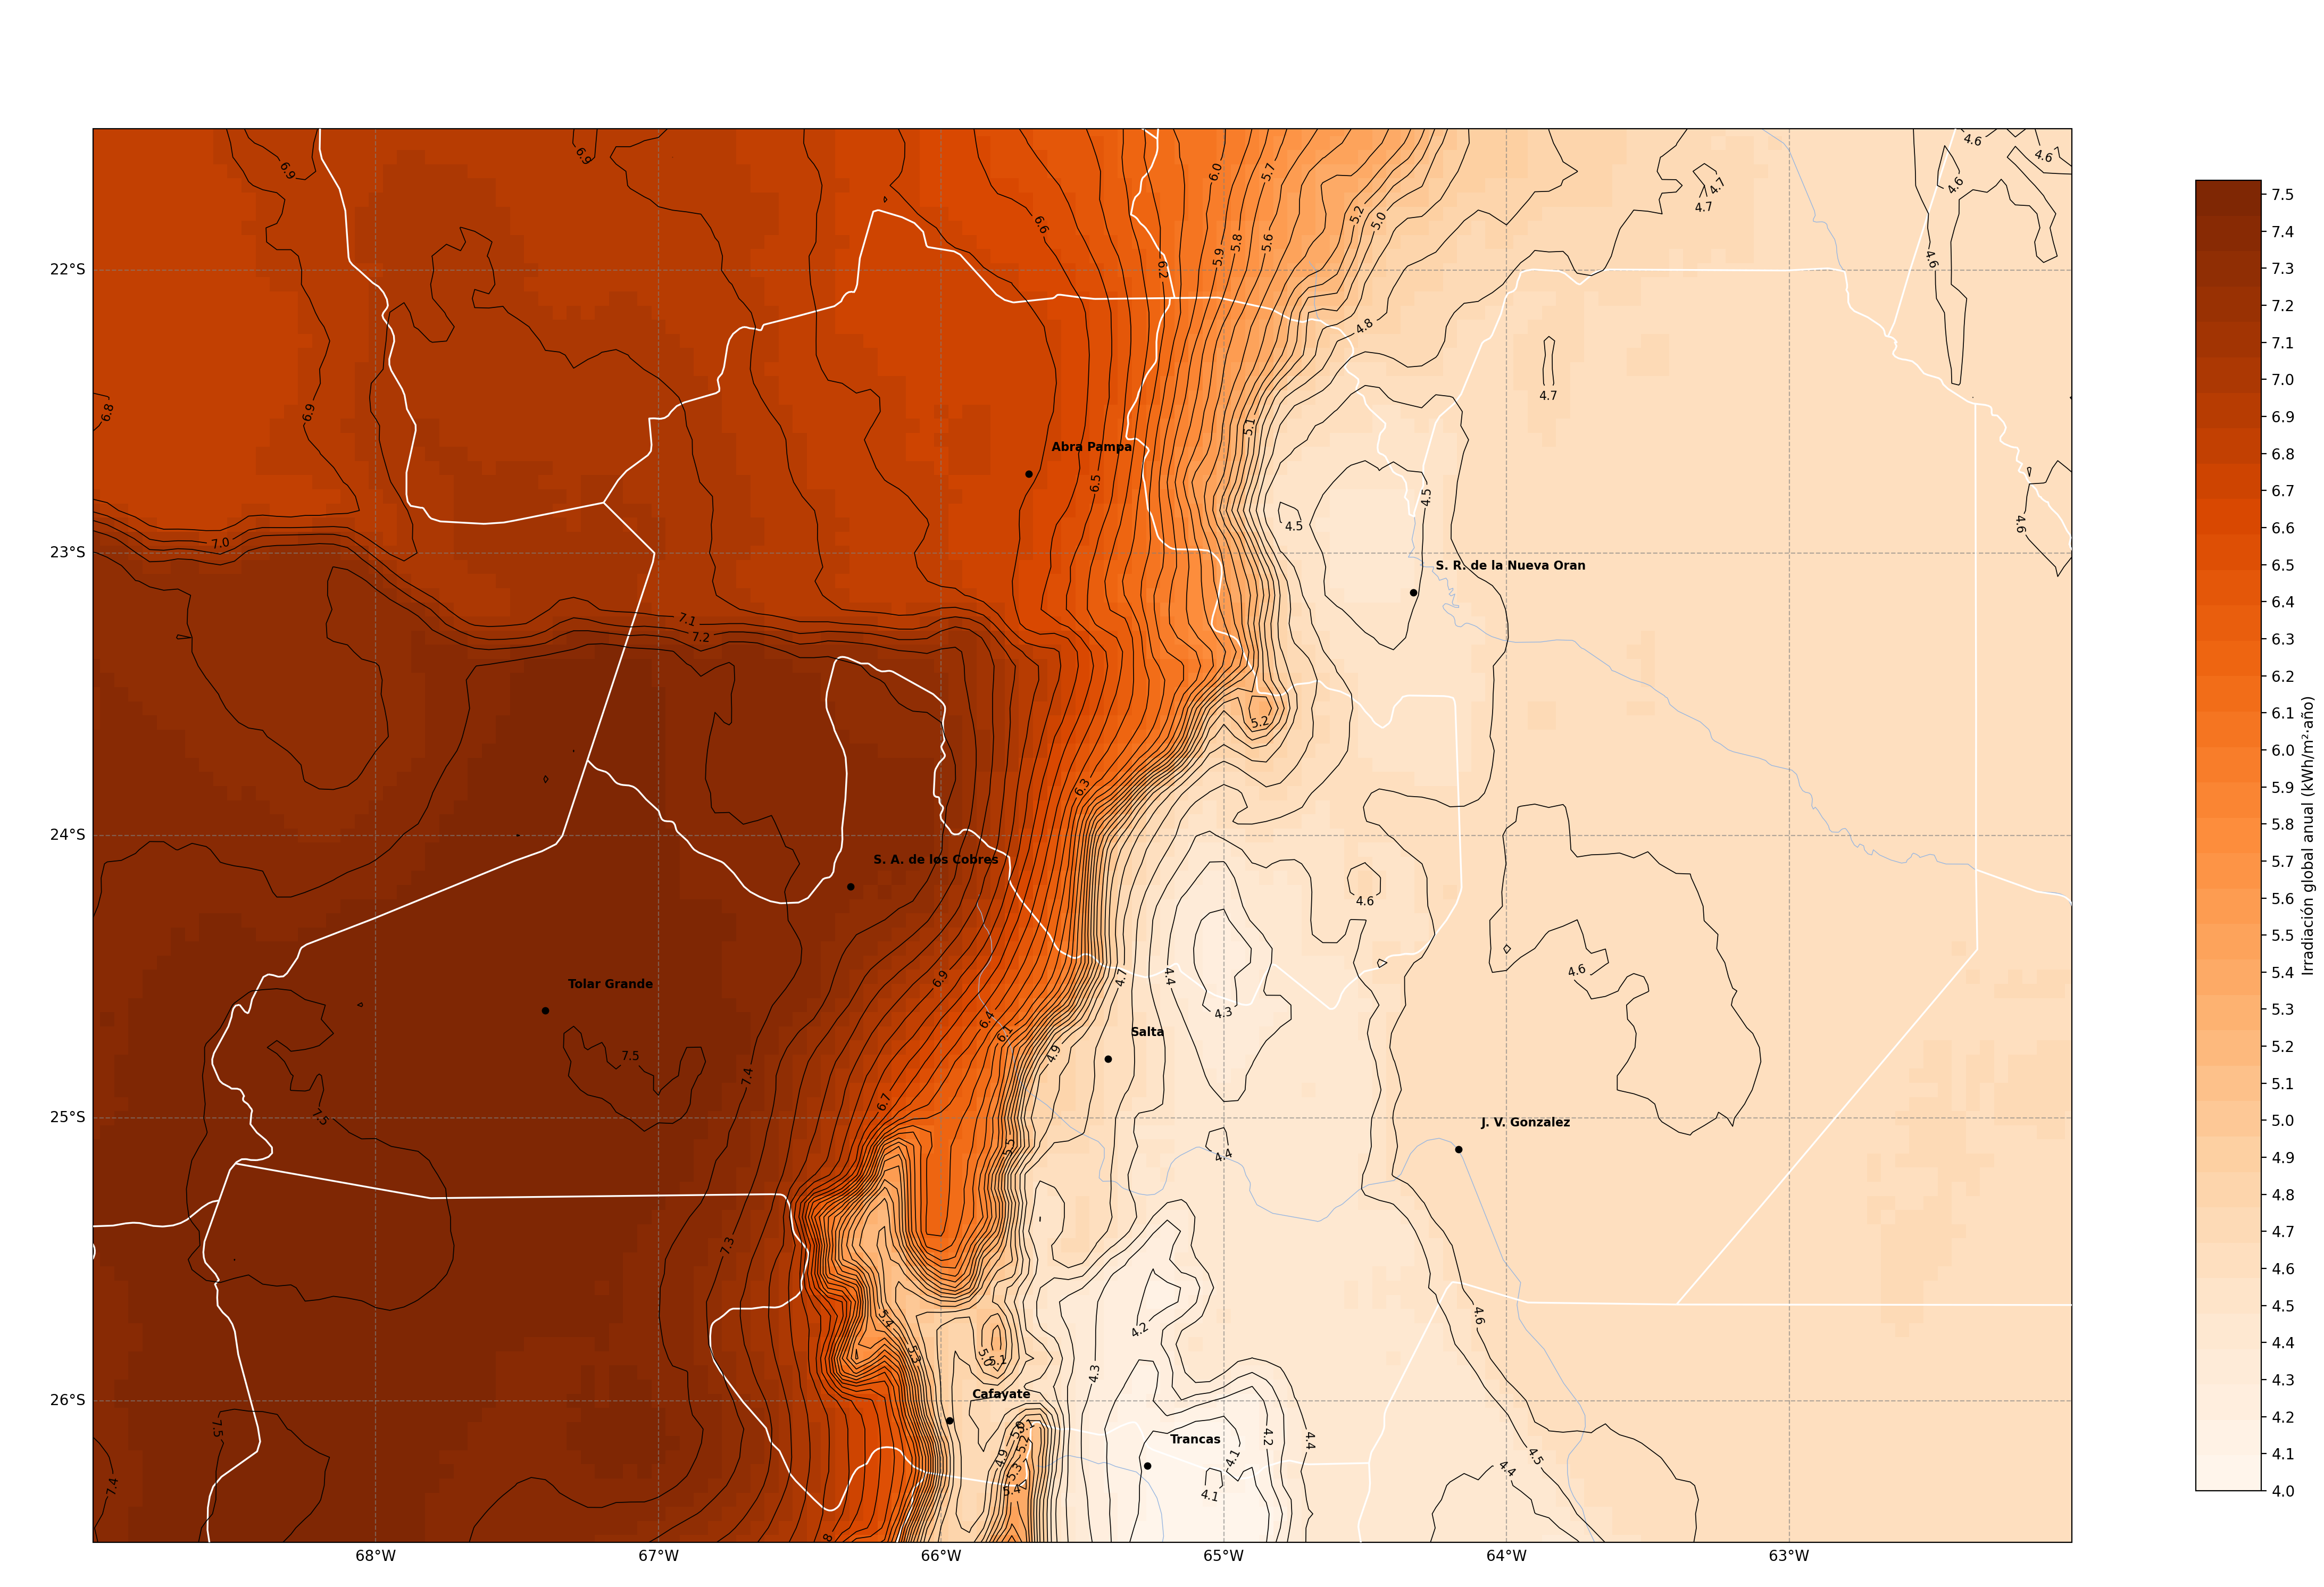
\includegraphics[width=0.99\textwidth]{figuras/Mapas/TMY.png}
    \caption{TMY }
    \label{fig:tmy}
\end{figure}